\chapter{Część praktyczna}


\begin{figure}[!ht]
    \centering
    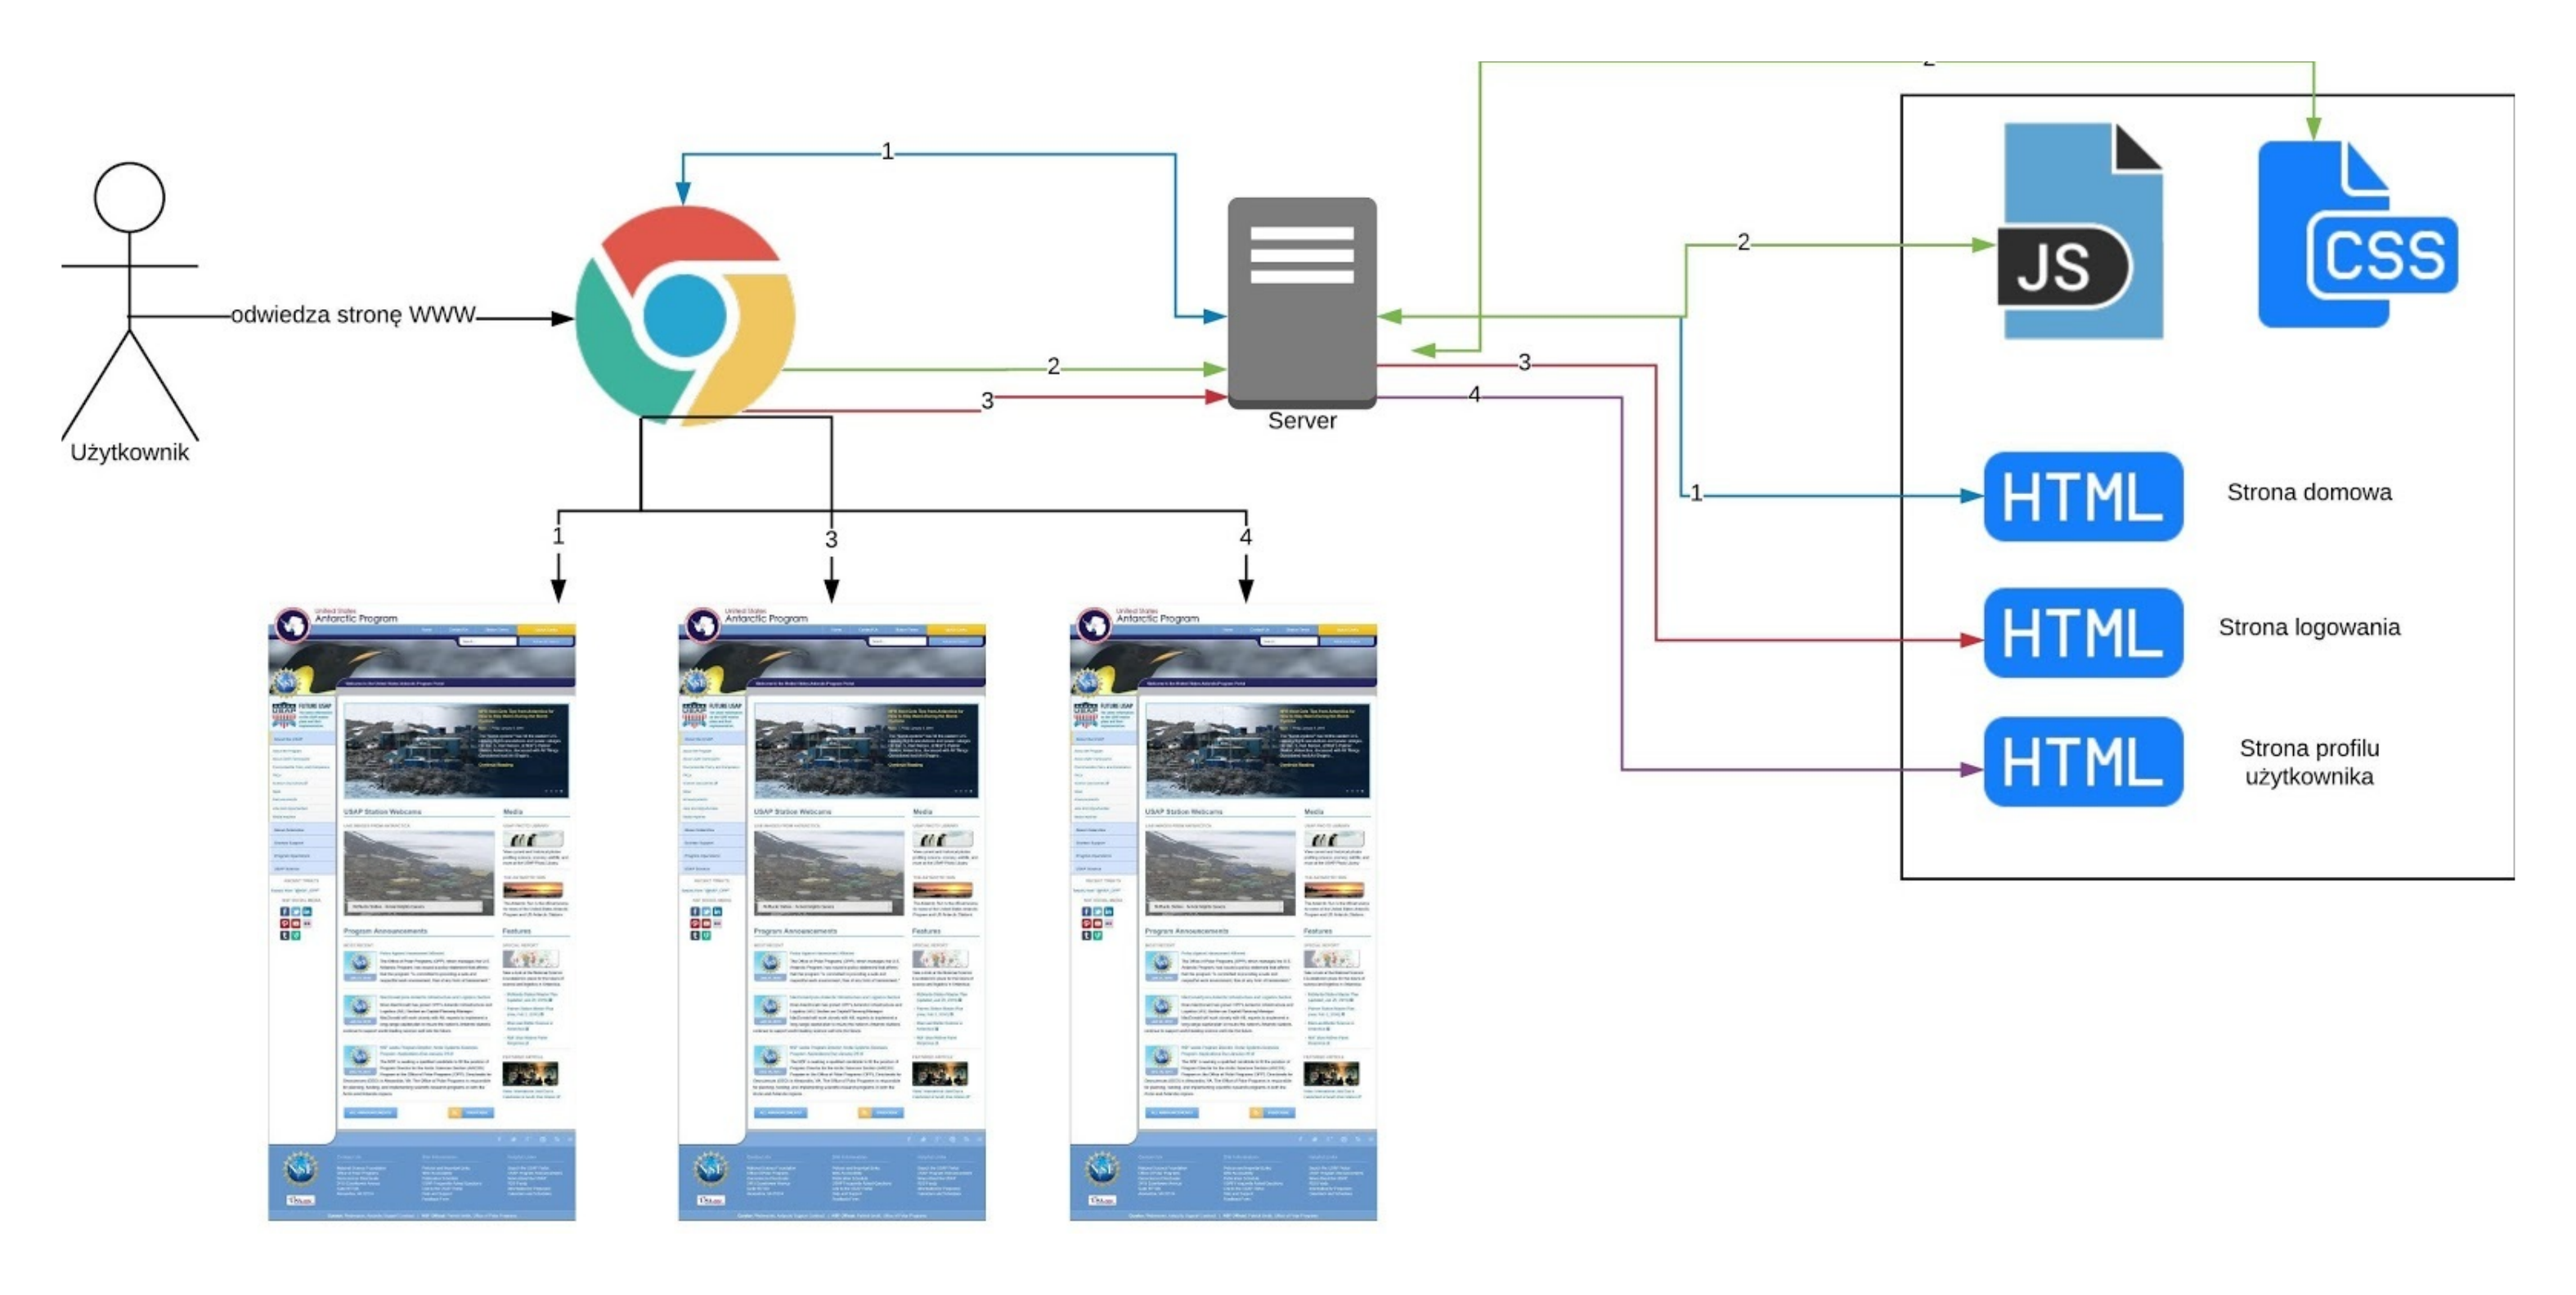
\includegraphics[width=12cm]{rysunek_7.png}
    \caption{Ilustracja przedstawiająca cykl życia statycznej strony internetowej}
    \label{fig:rysunek_7}
\end{figure}

\begin{figure}[!ht]
    \centering
    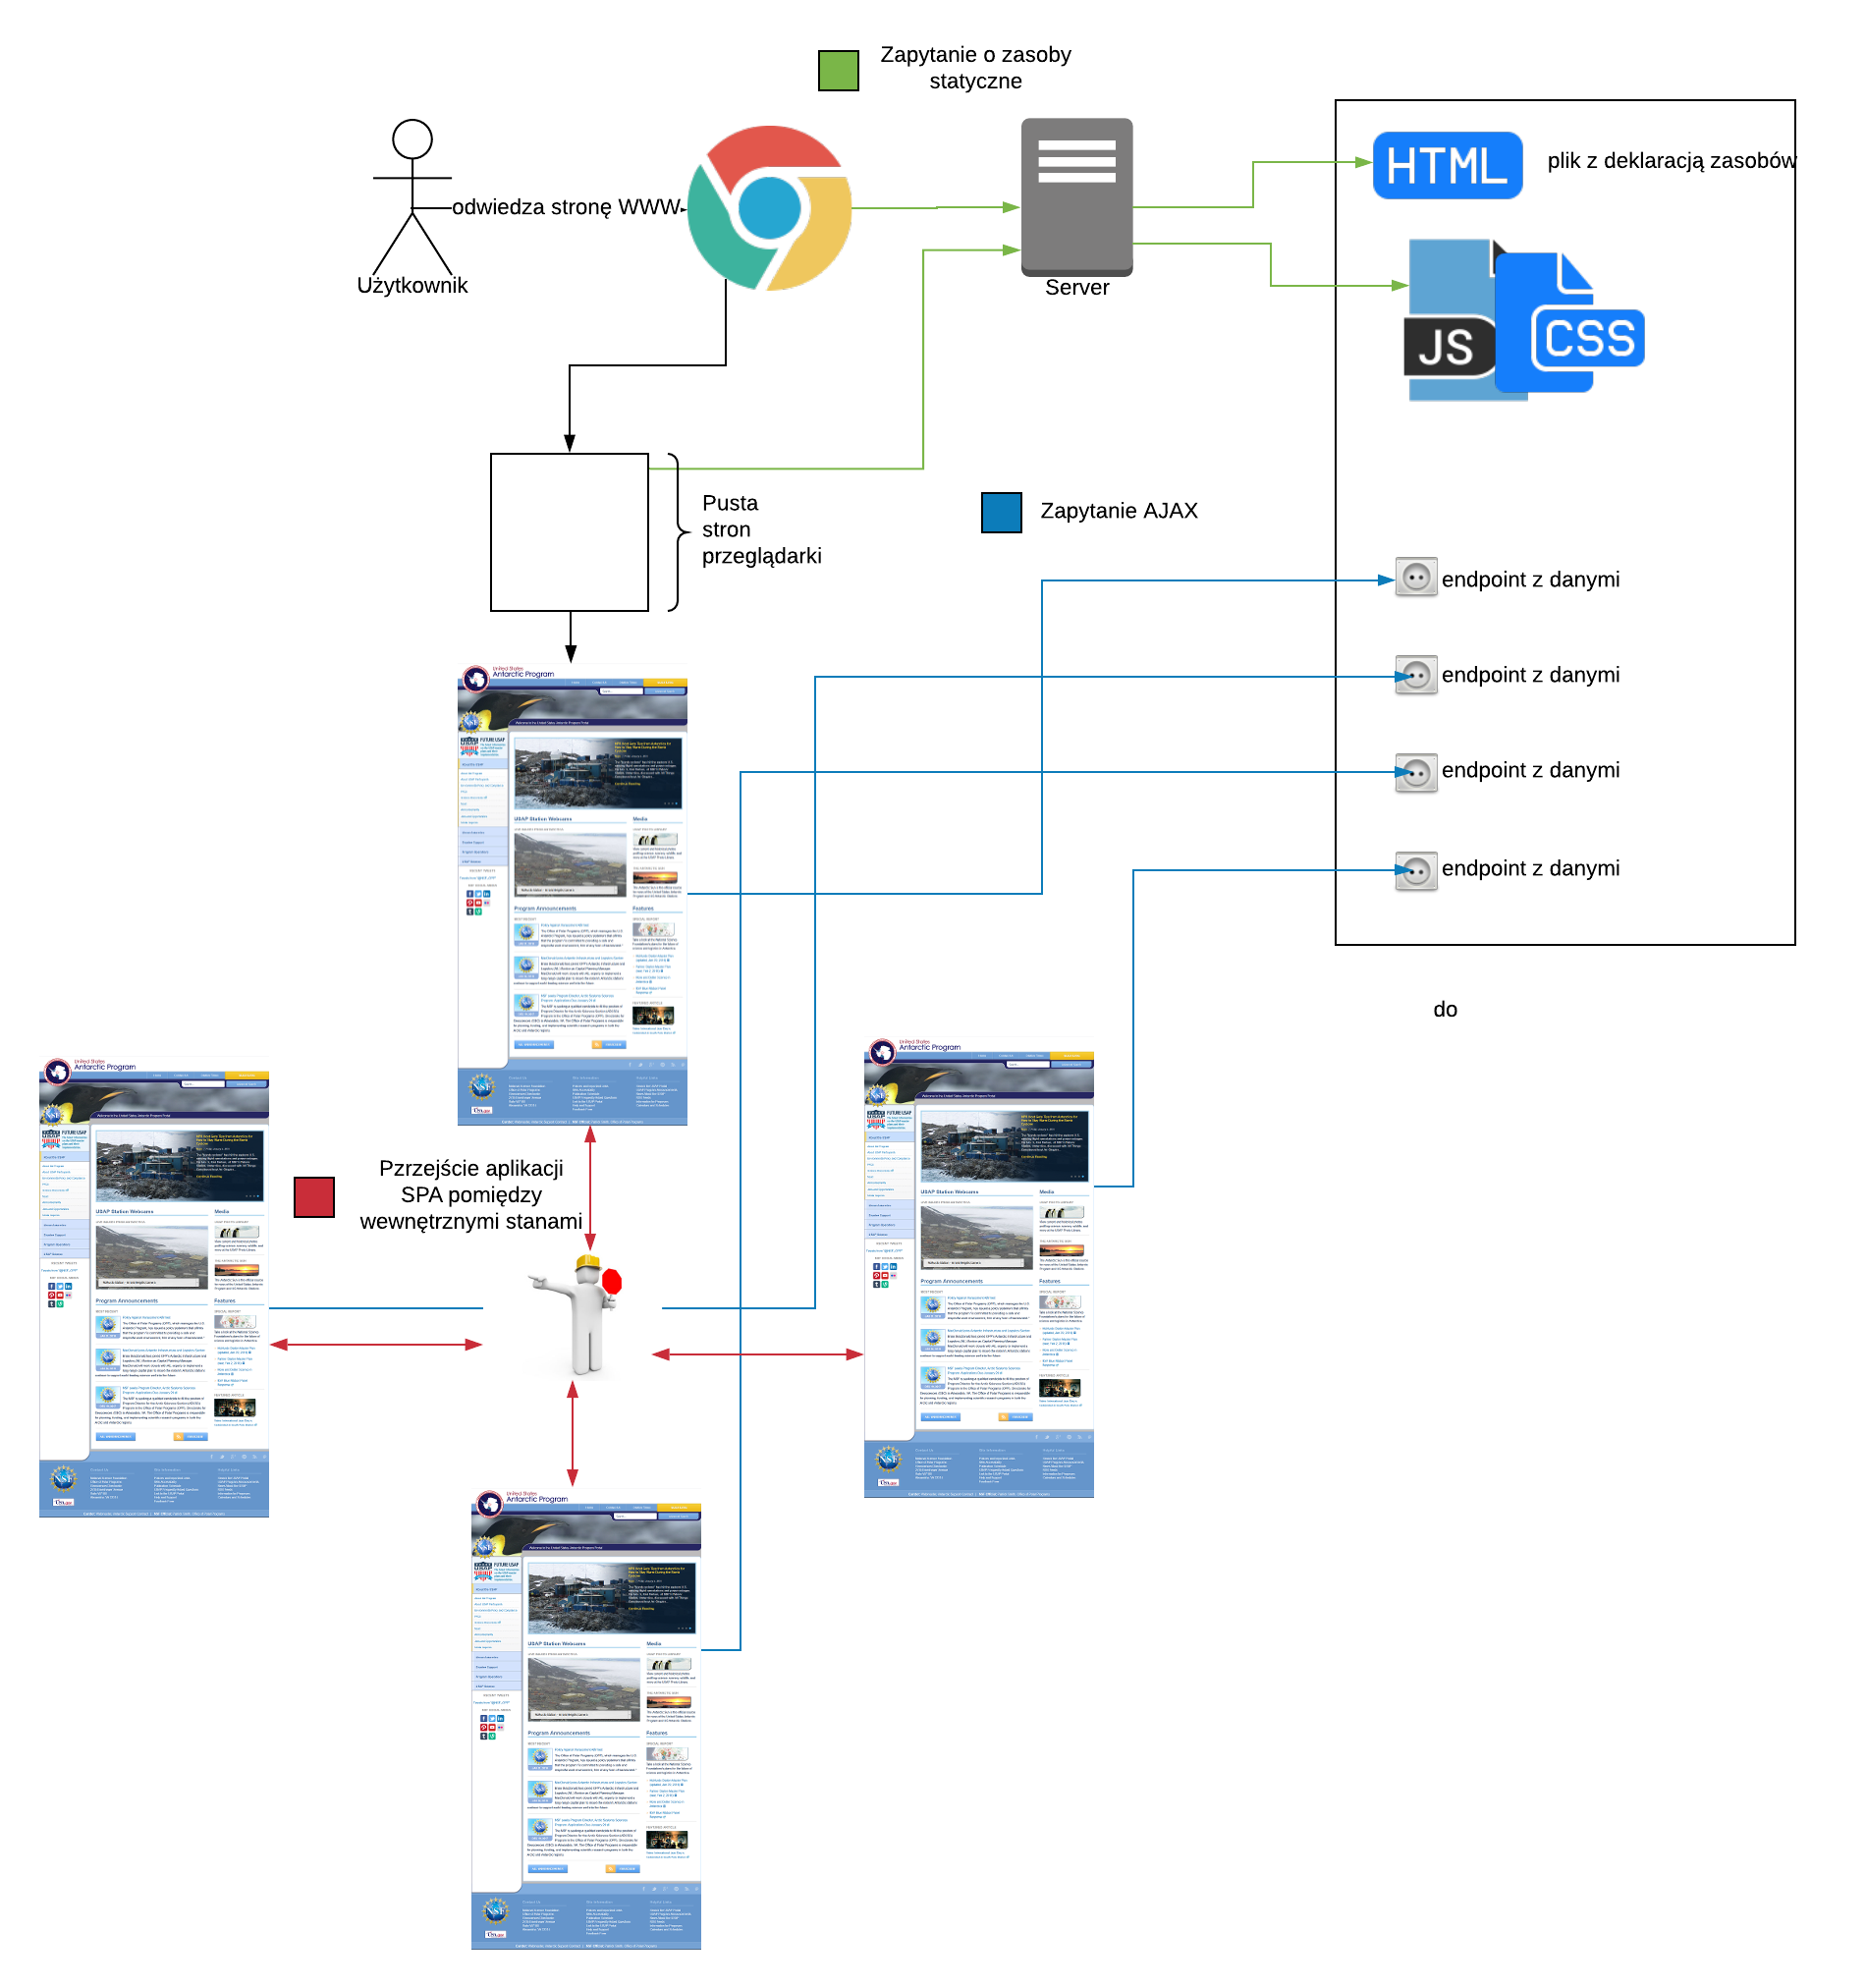
\includegraphics[width=12cm]{rysunek_8.png}
    \caption{Ilustracja przedstawiająca cykl działania aplikacji SPA}
    \label{fig:rysunek_8}
\end{figure}

\begin{figure}[!ht]
    \centering
    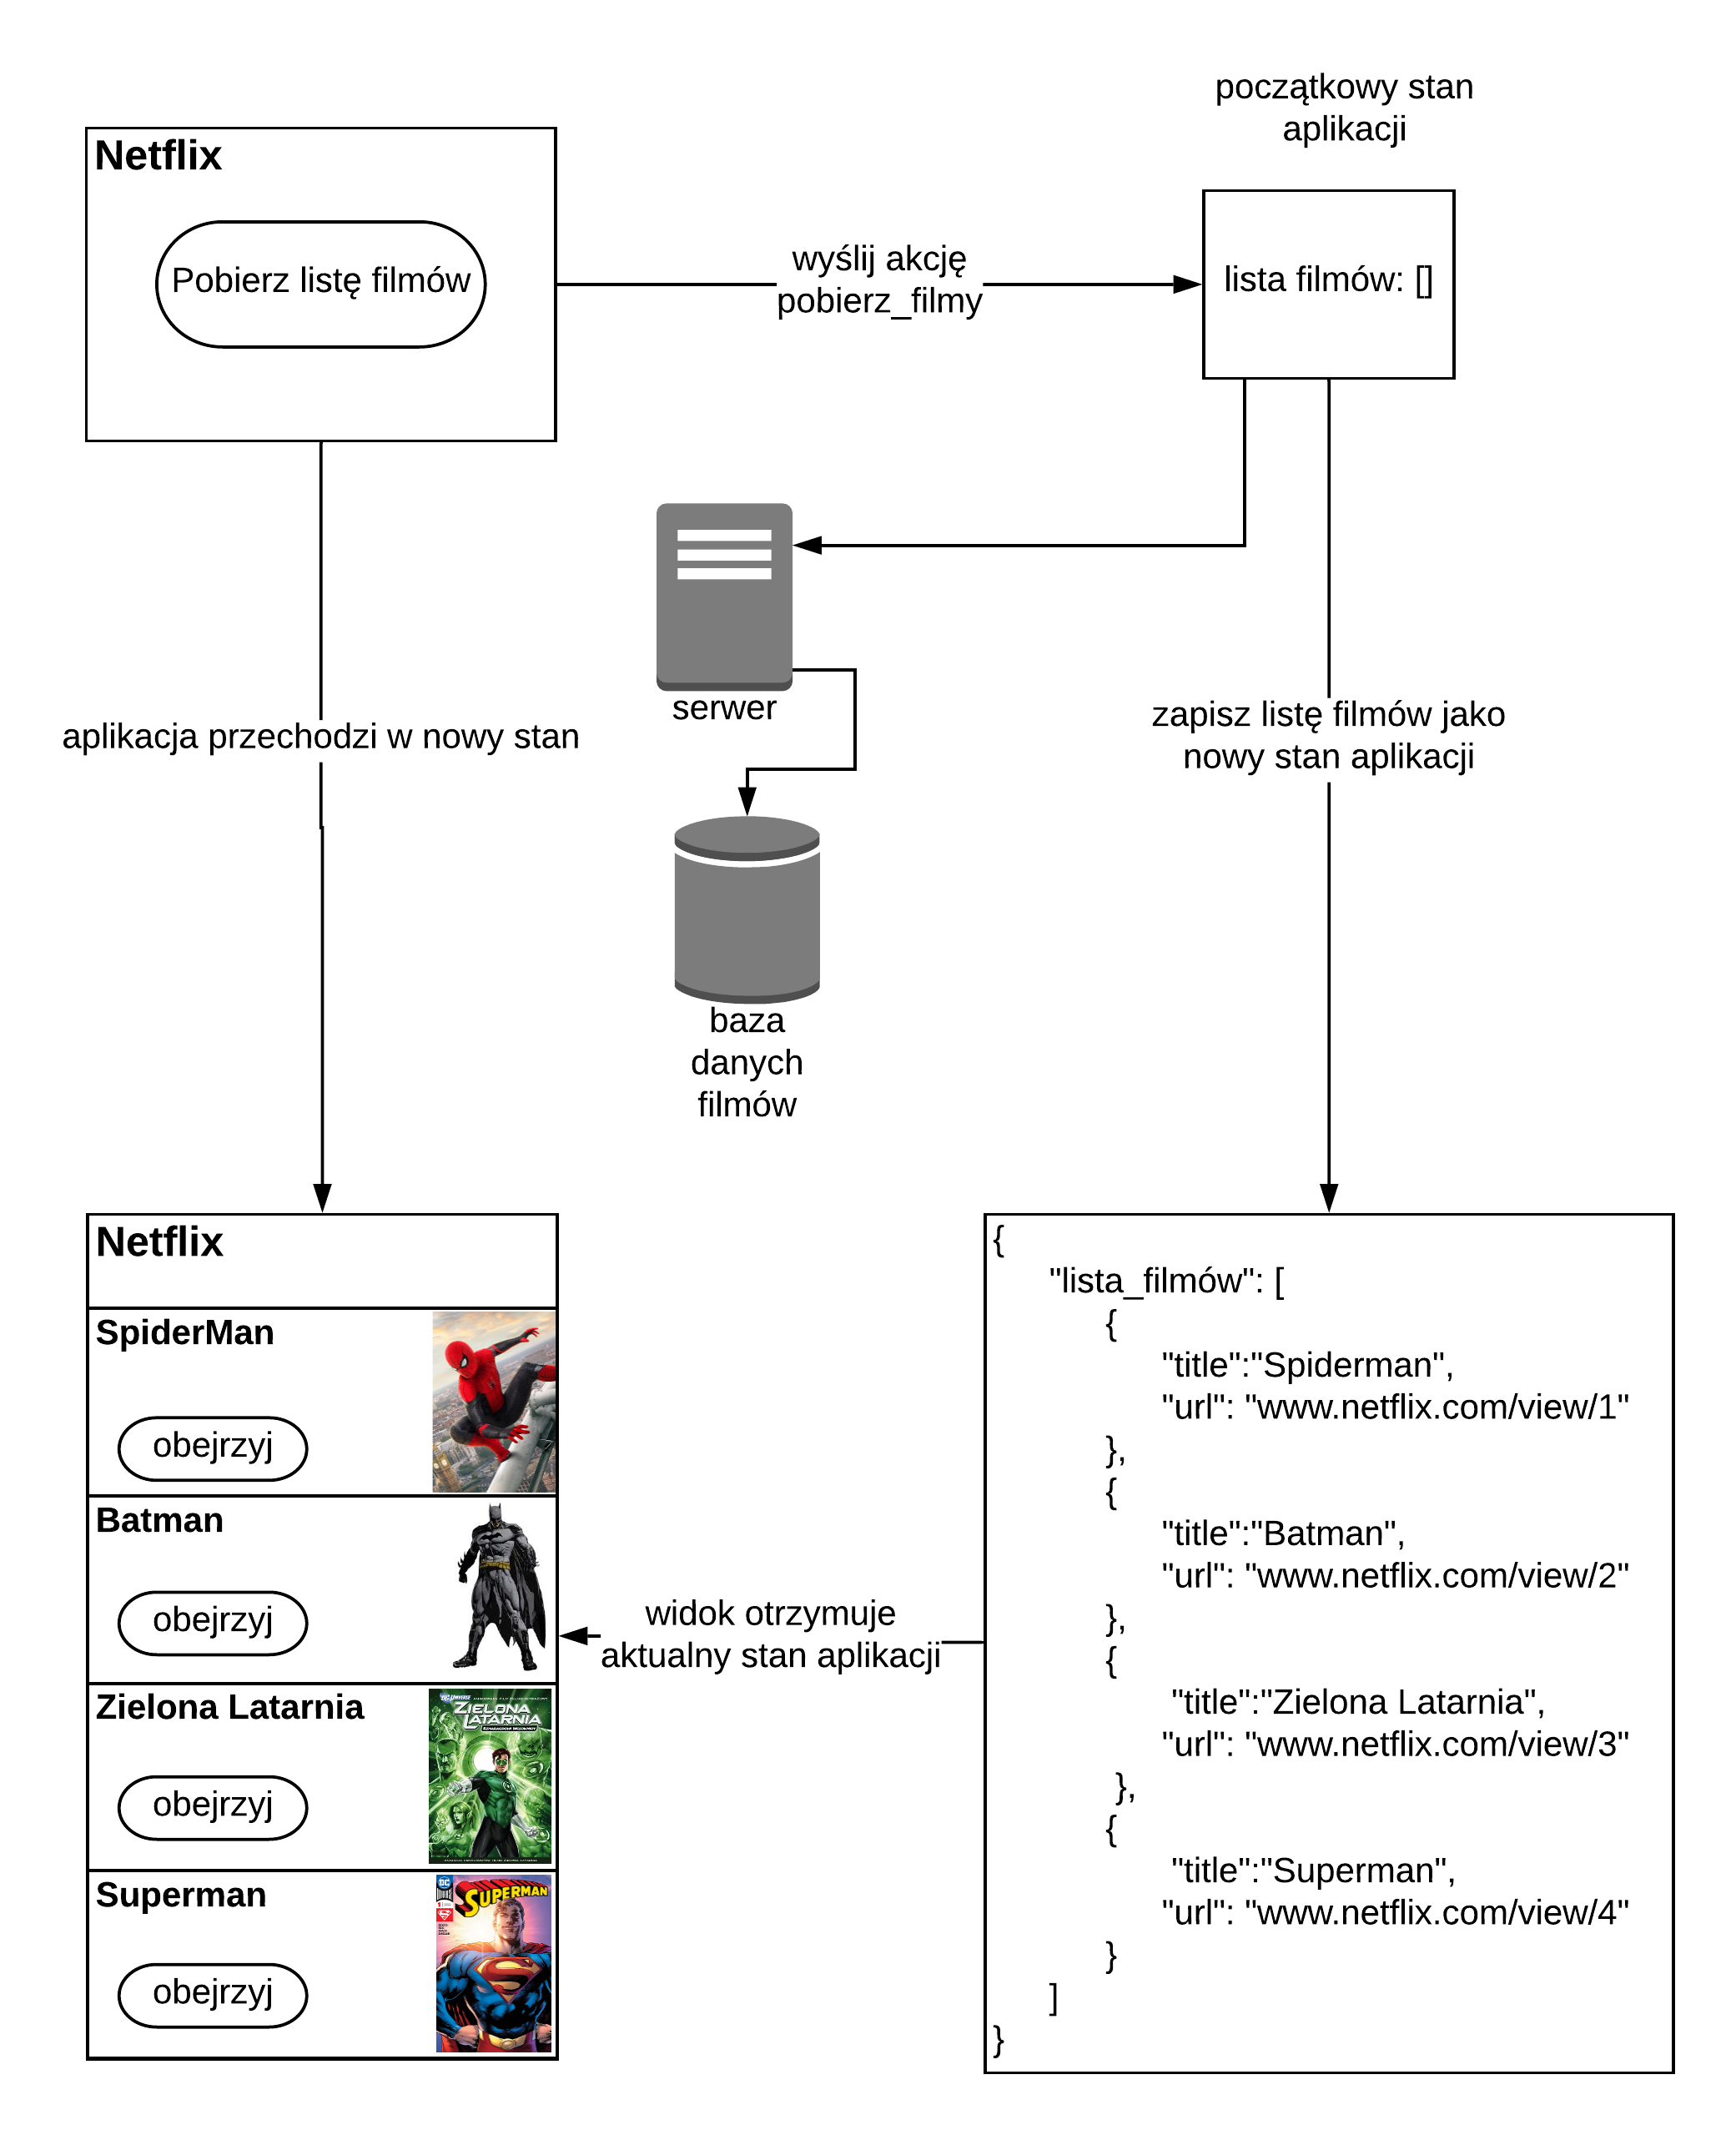
\includegraphics[width=12cm]{rysunek_9.png}
    \caption{Grafika przedstawiająca mechanizm działania aplikacji dynamicznych}
    \label{fig:rysunek_9}
\end{figure}

\begin{figure}[!ht]
    \centering
    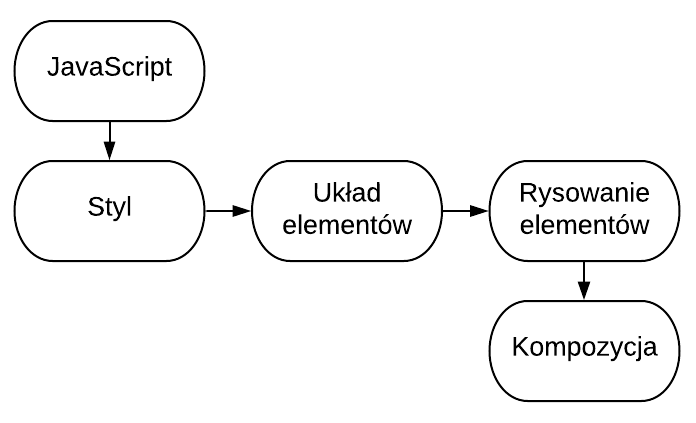
\includegraphics[width=12cm]{rysunek_10.png}
    \caption{Grafika przedstawiająca kolejność faz renderowania w przeglądarce}
    \label{fig:rysunek_10}
\end{figure}

\begin{figure}[!ht]
    \centering
    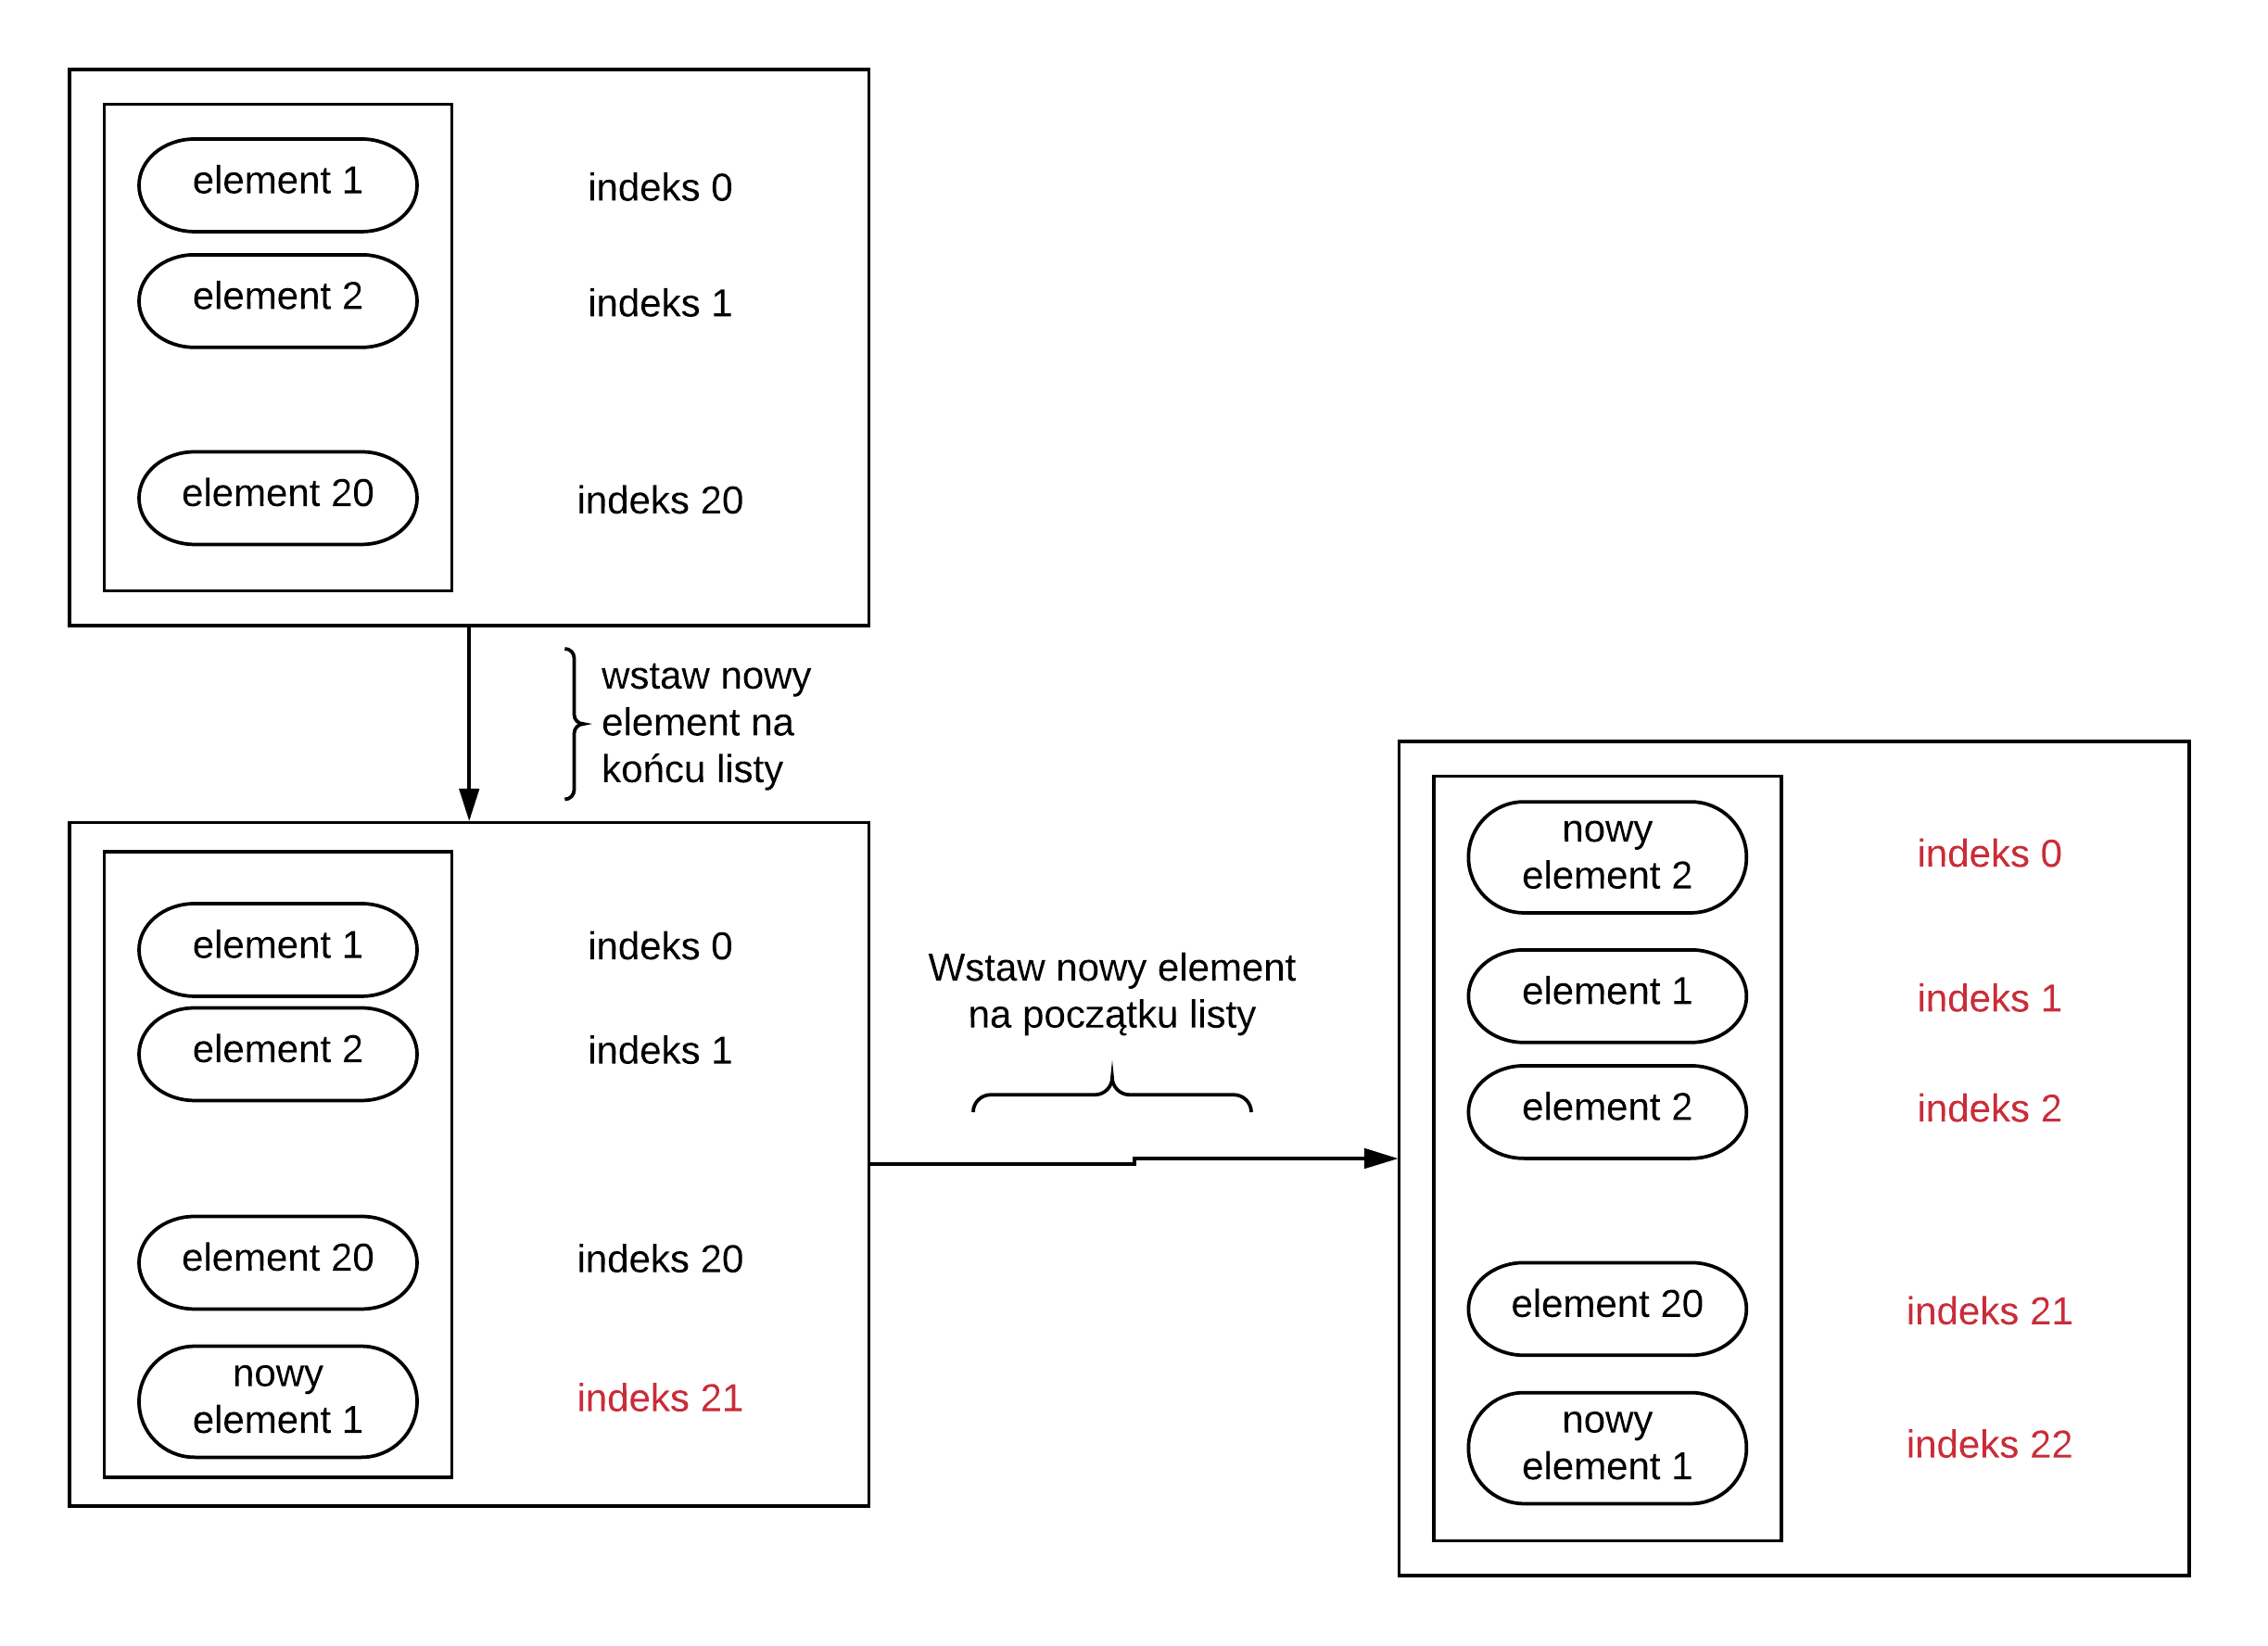
\includegraphics[width=12cm]{rysunek_11.png}
    \caption{Ilustracja przedstawiająca problem dopisywania elementu na koniec listy}
    \label{fig:rysunek_11}
\end{figure}

\begin{figure}[!ht]
    \centering
    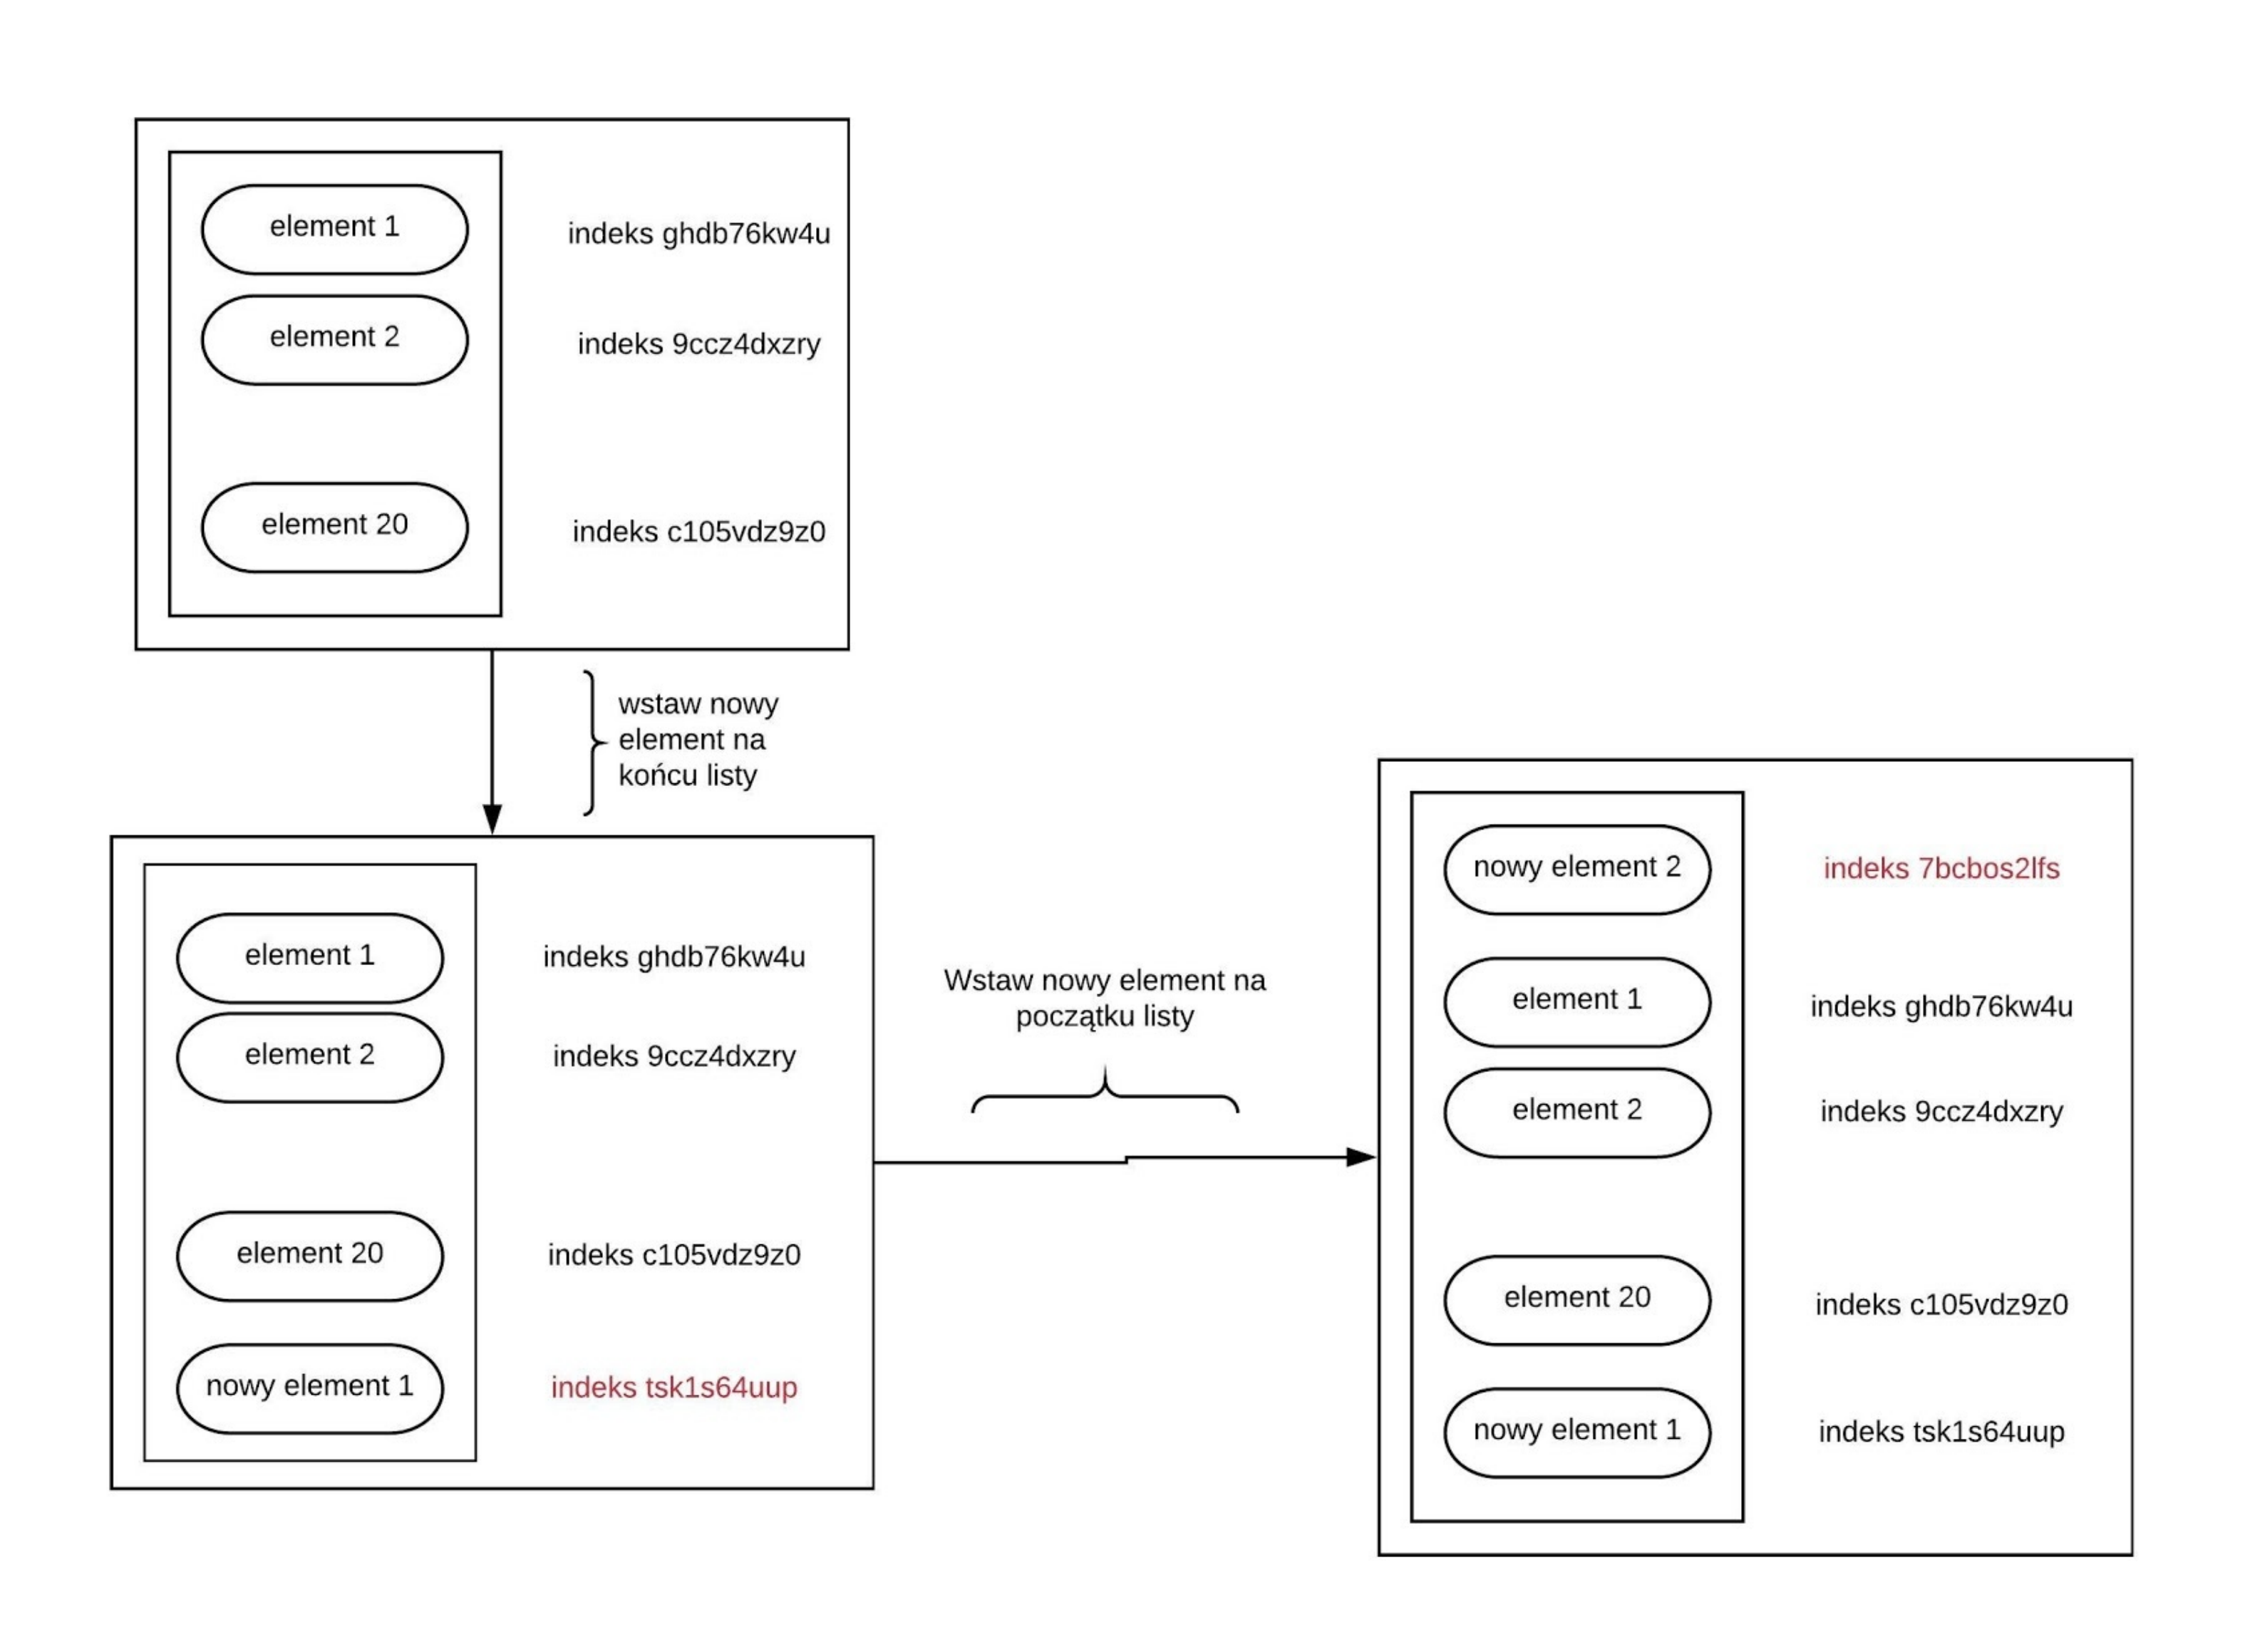
\includegraphics[width=12cm]{rysunek_12.png}
    \caption{Ilustracja przedstawiająca problem dopisywania elementów na początek listy}
    \label{fig:rysunek_12}
\end{figure}

\begin{figure}[!ht]
    \centering
    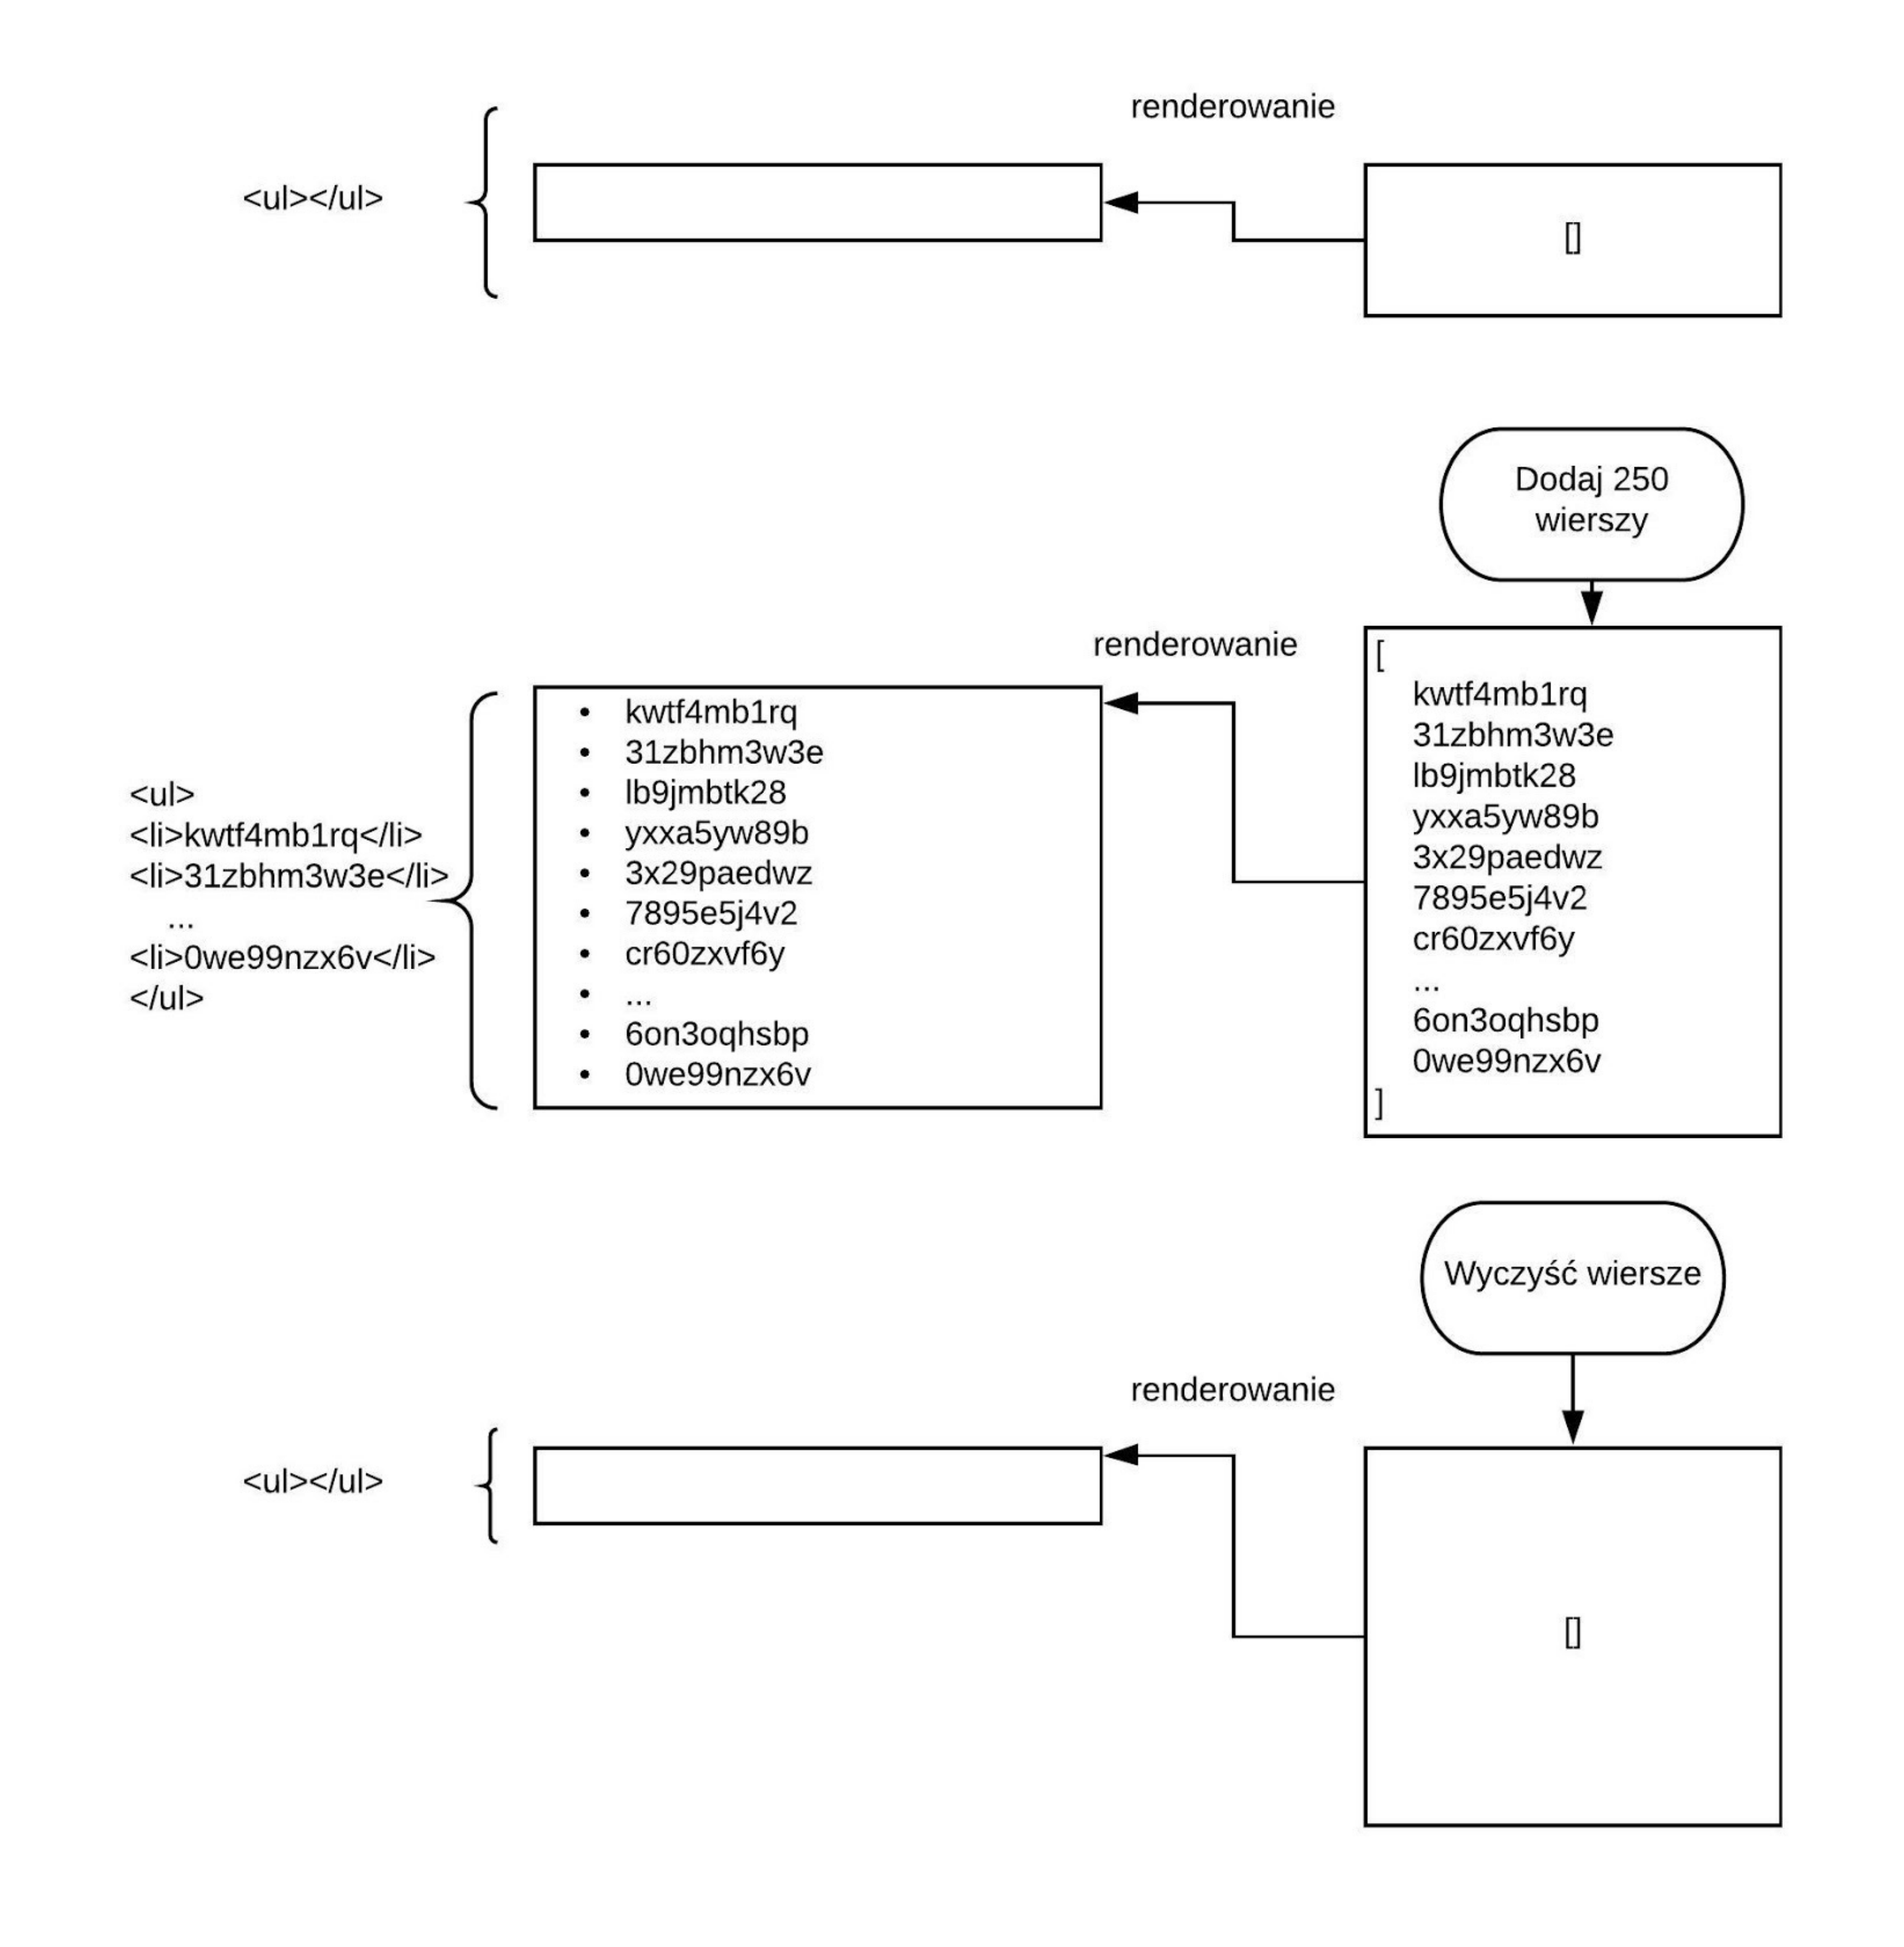
\includegraphics[width=12cm]{rysunek_13.png}
    \caption{Ilustracja mechanizmu przebiegu badania}
    \label{fig:rysunek_13}
\end{figure}

\begin{figure}[!ht]
    \centering
    
\includegraphics[width=12cm]{rysunek_14.png}
    \caption{Grafika przedstawiająca zaimplementowane przyciski w aplikacji}
    \label{fig:rysunek_14}
\end{figure}

\begin{figure}[!ht]
    \centering
    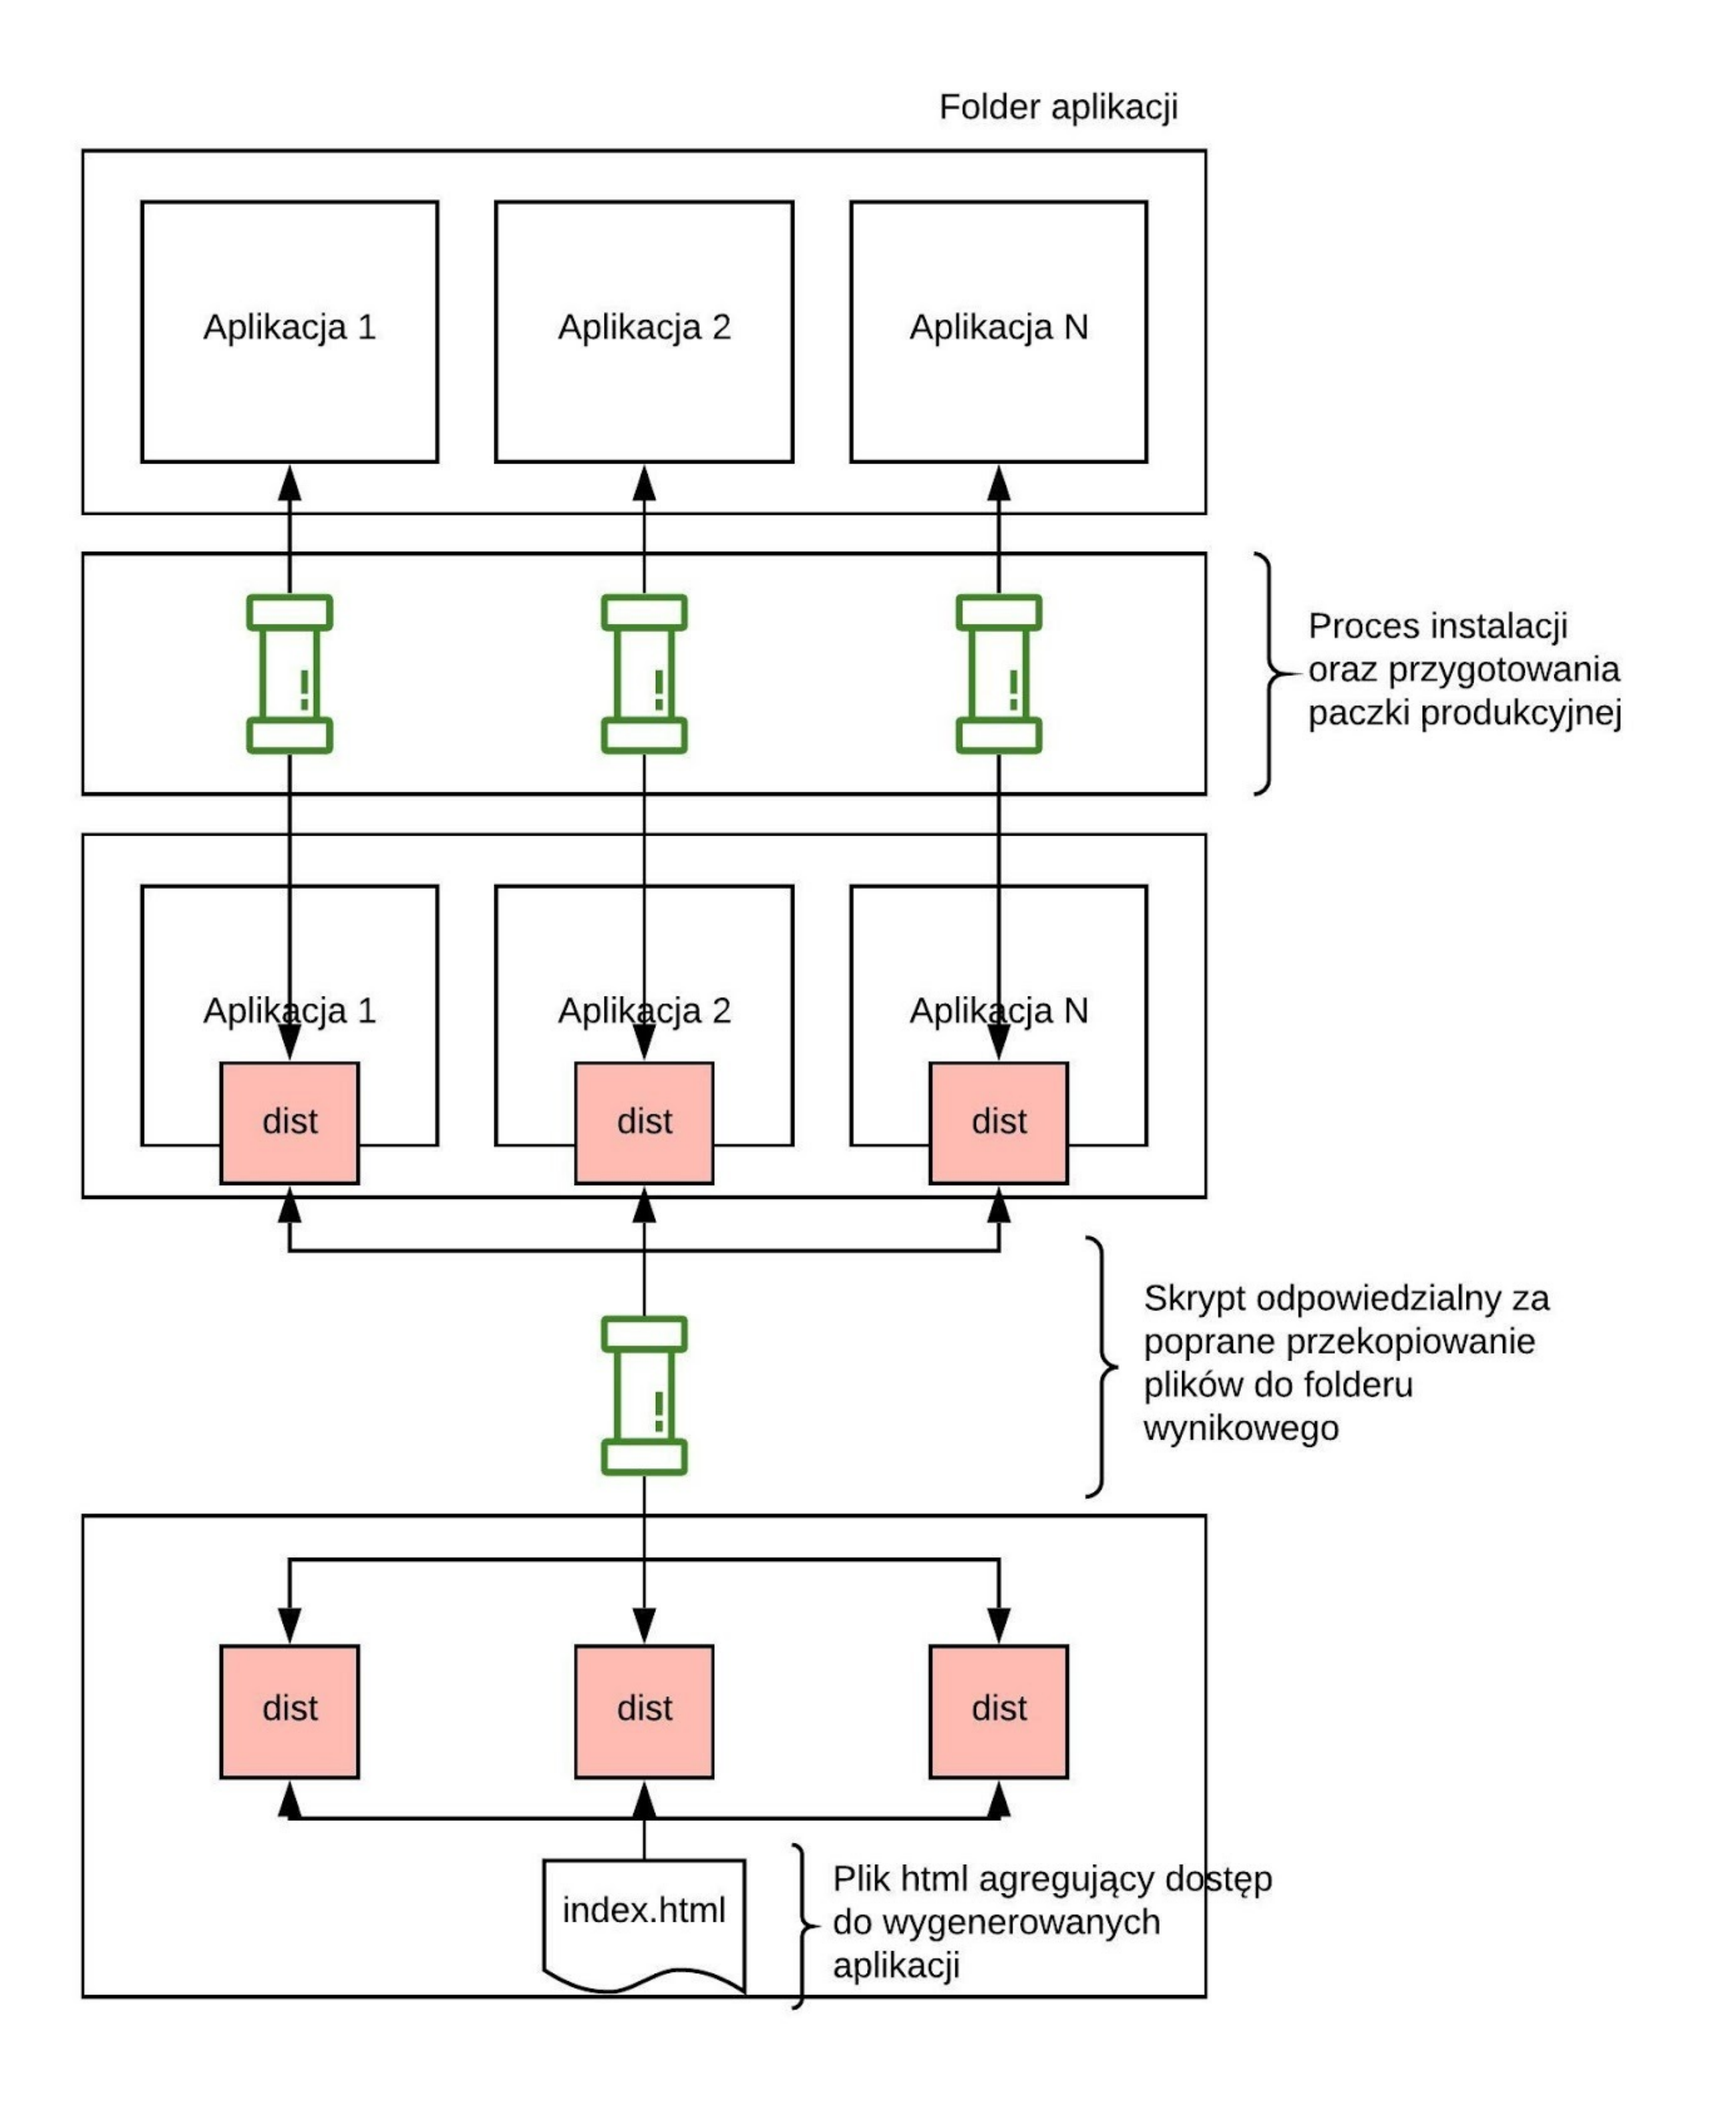
\includegraphics[width=12cm]{rysunek_15.png}
    \caption{Ilustracja procesu przygotowania aplikacji do konteneryzacji}
    \label{fig:rysunek_15}
\end{figure}

\begin{figure}[!ht]
    \centering
    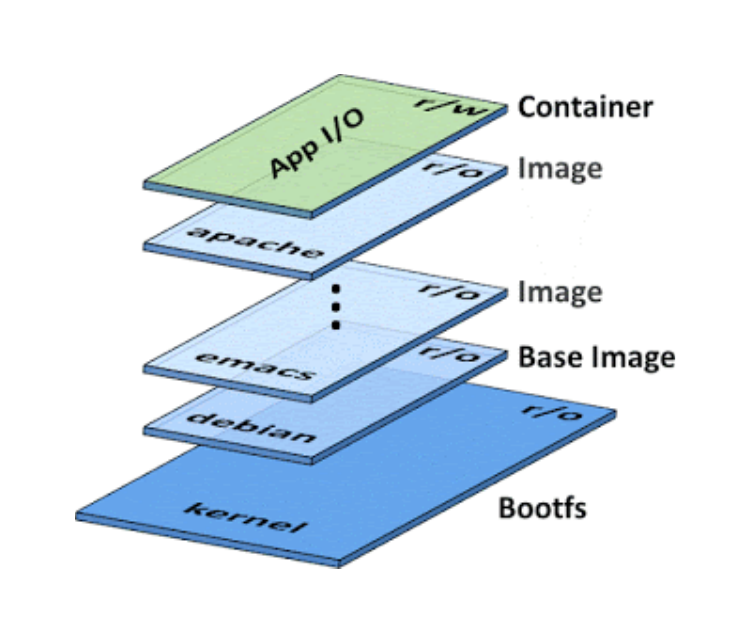
\includegraphics[width=12cm]{rysunek_16.png}
    \caption{Ilustracja przedstawiająca warstwy składające się na  przykładowy obraz dockera}
    \label{fig:rysunek_16}
\end{figure}

\begin{figure}[!ht]
    \centering
    
\includegraphics[width=12cm]{rysunek_17.png}
    \caption{Grafika przedstawiająca plik index.html wraz z dostępnymi aplikacjami do badania}
    \label{fig:rysunek_17}
\end{figure}

\begin{figure}[!ht]
    \centering
    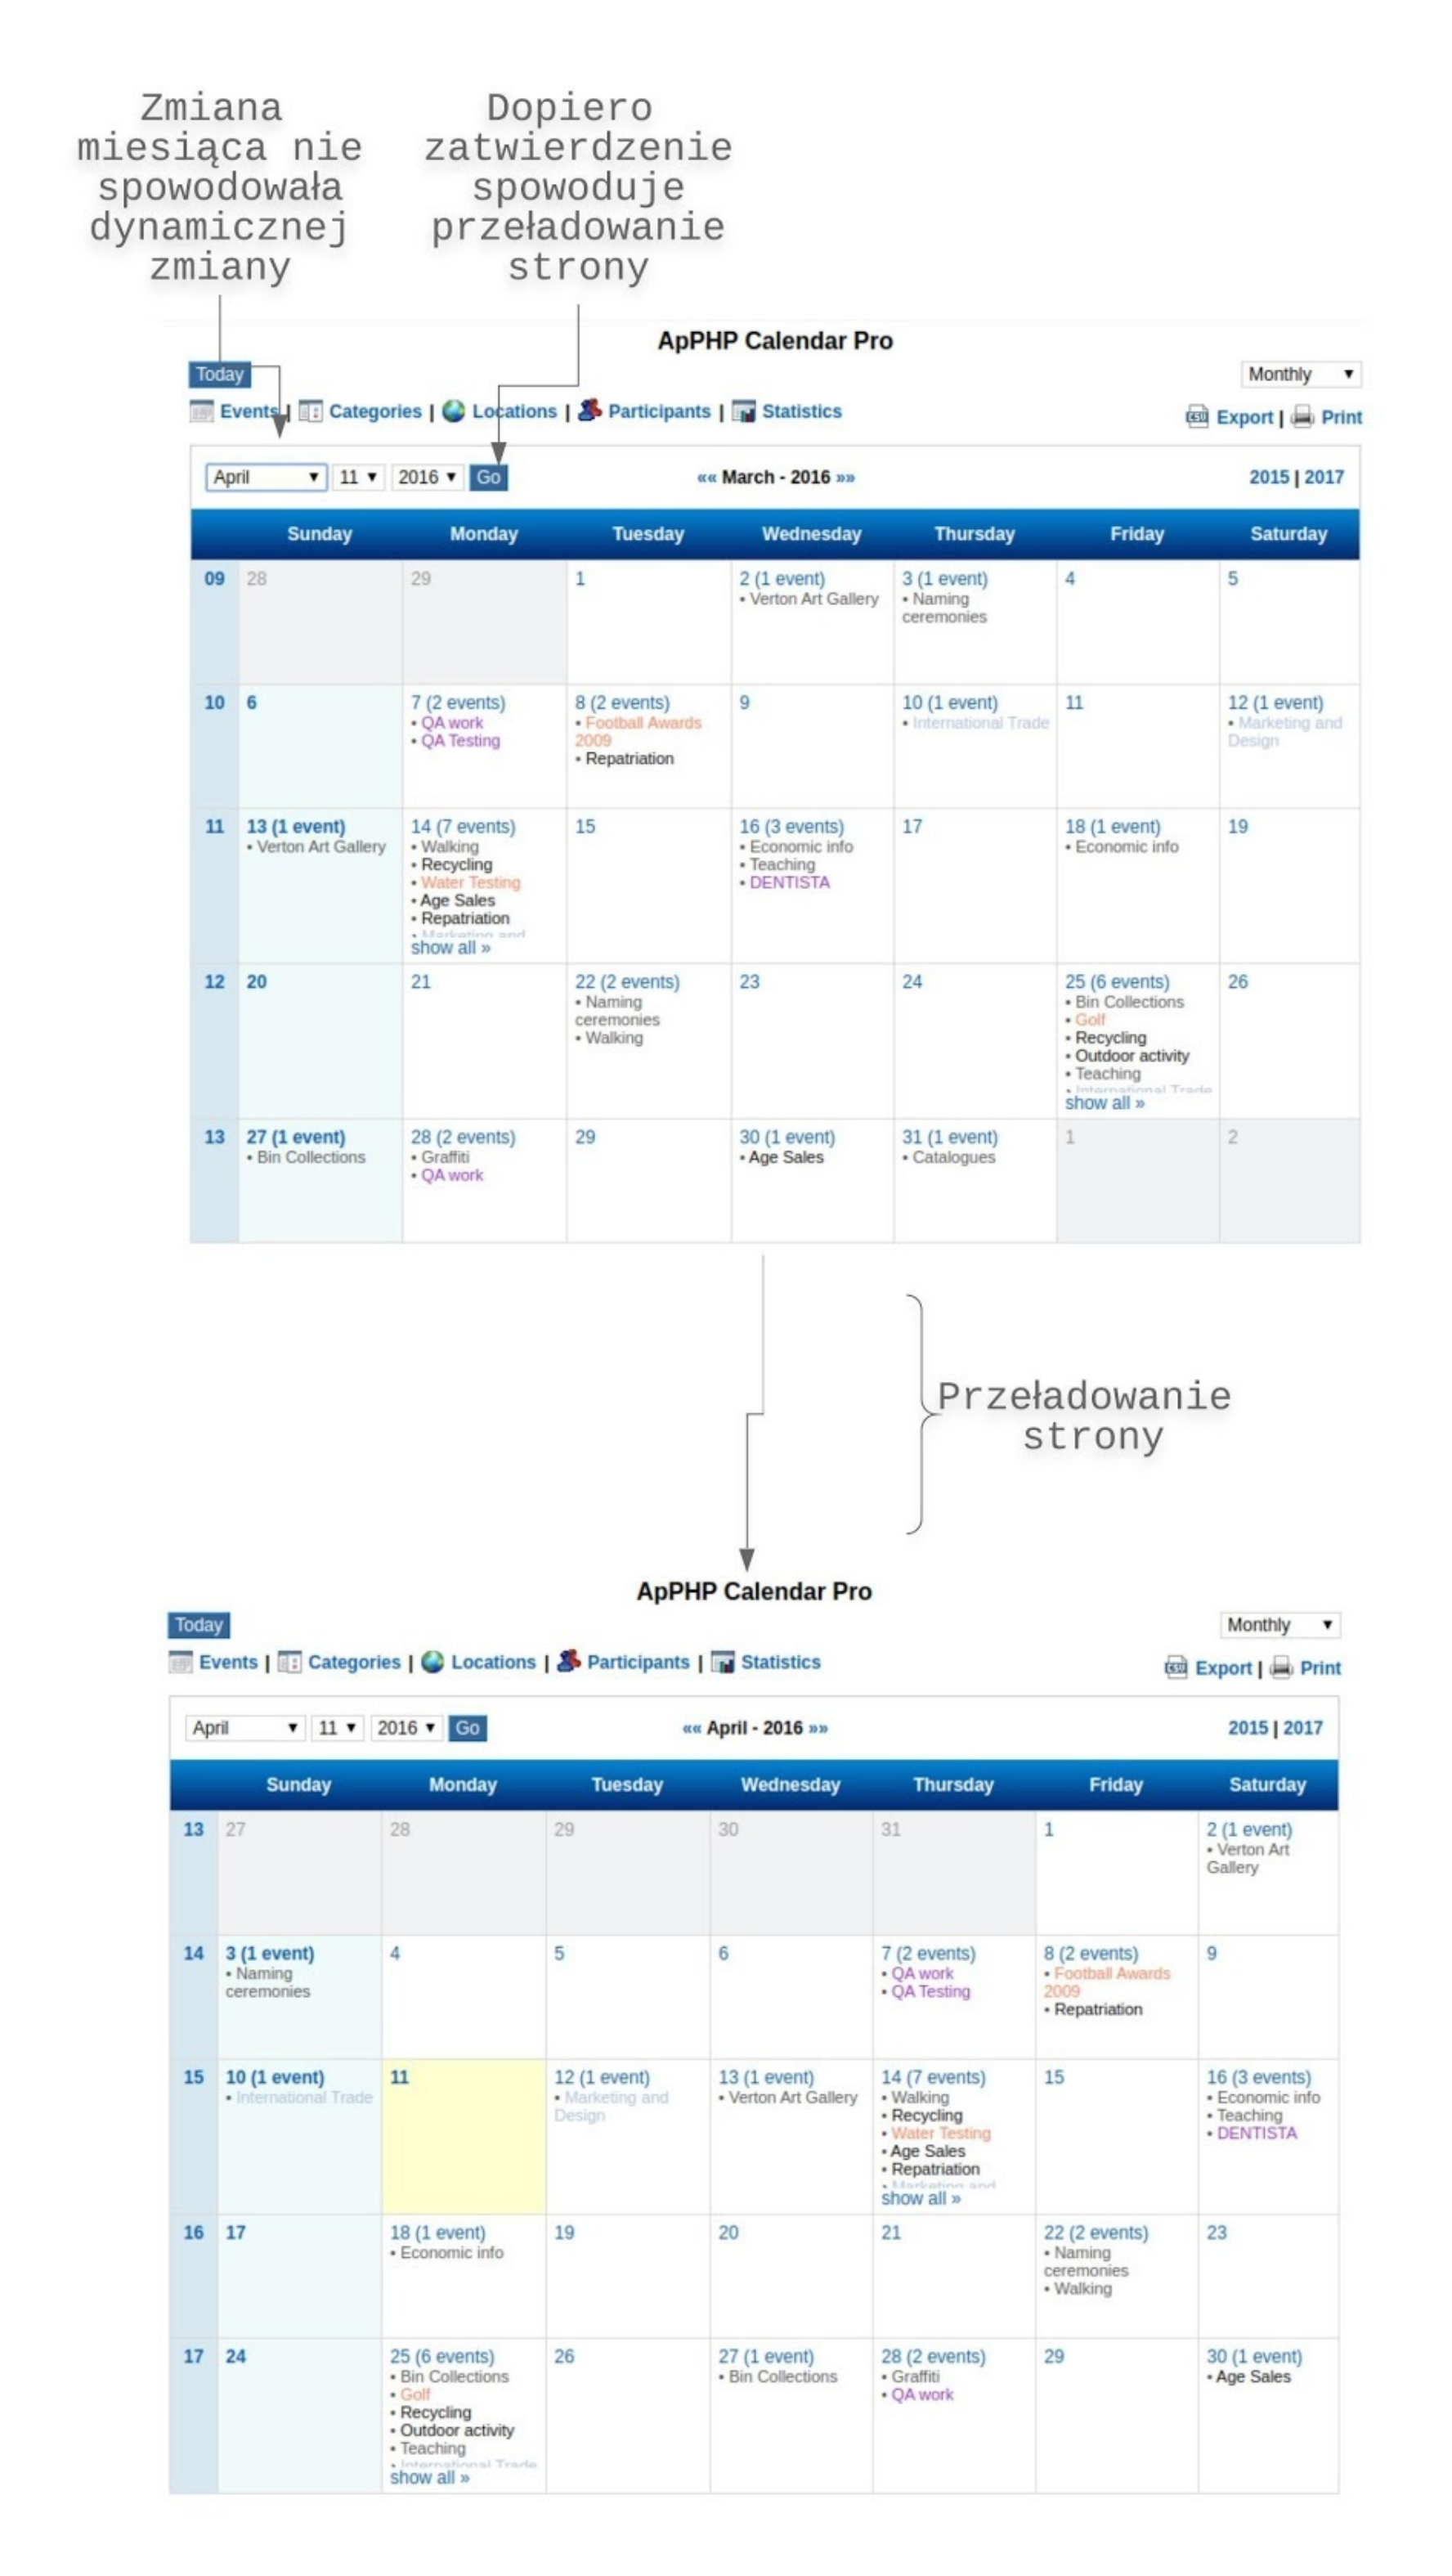
\includegraphics[width=12cm]{rysunek_18.png}
    \caption{Ilustracja mechanizmu działania strony statycznej na przykładzie aplikacji kalendarza przy użyciu języka PHP}
    \label{fig:rysunek_18}
\end{figure}

\begin{figure}[!ht]
    \centering
    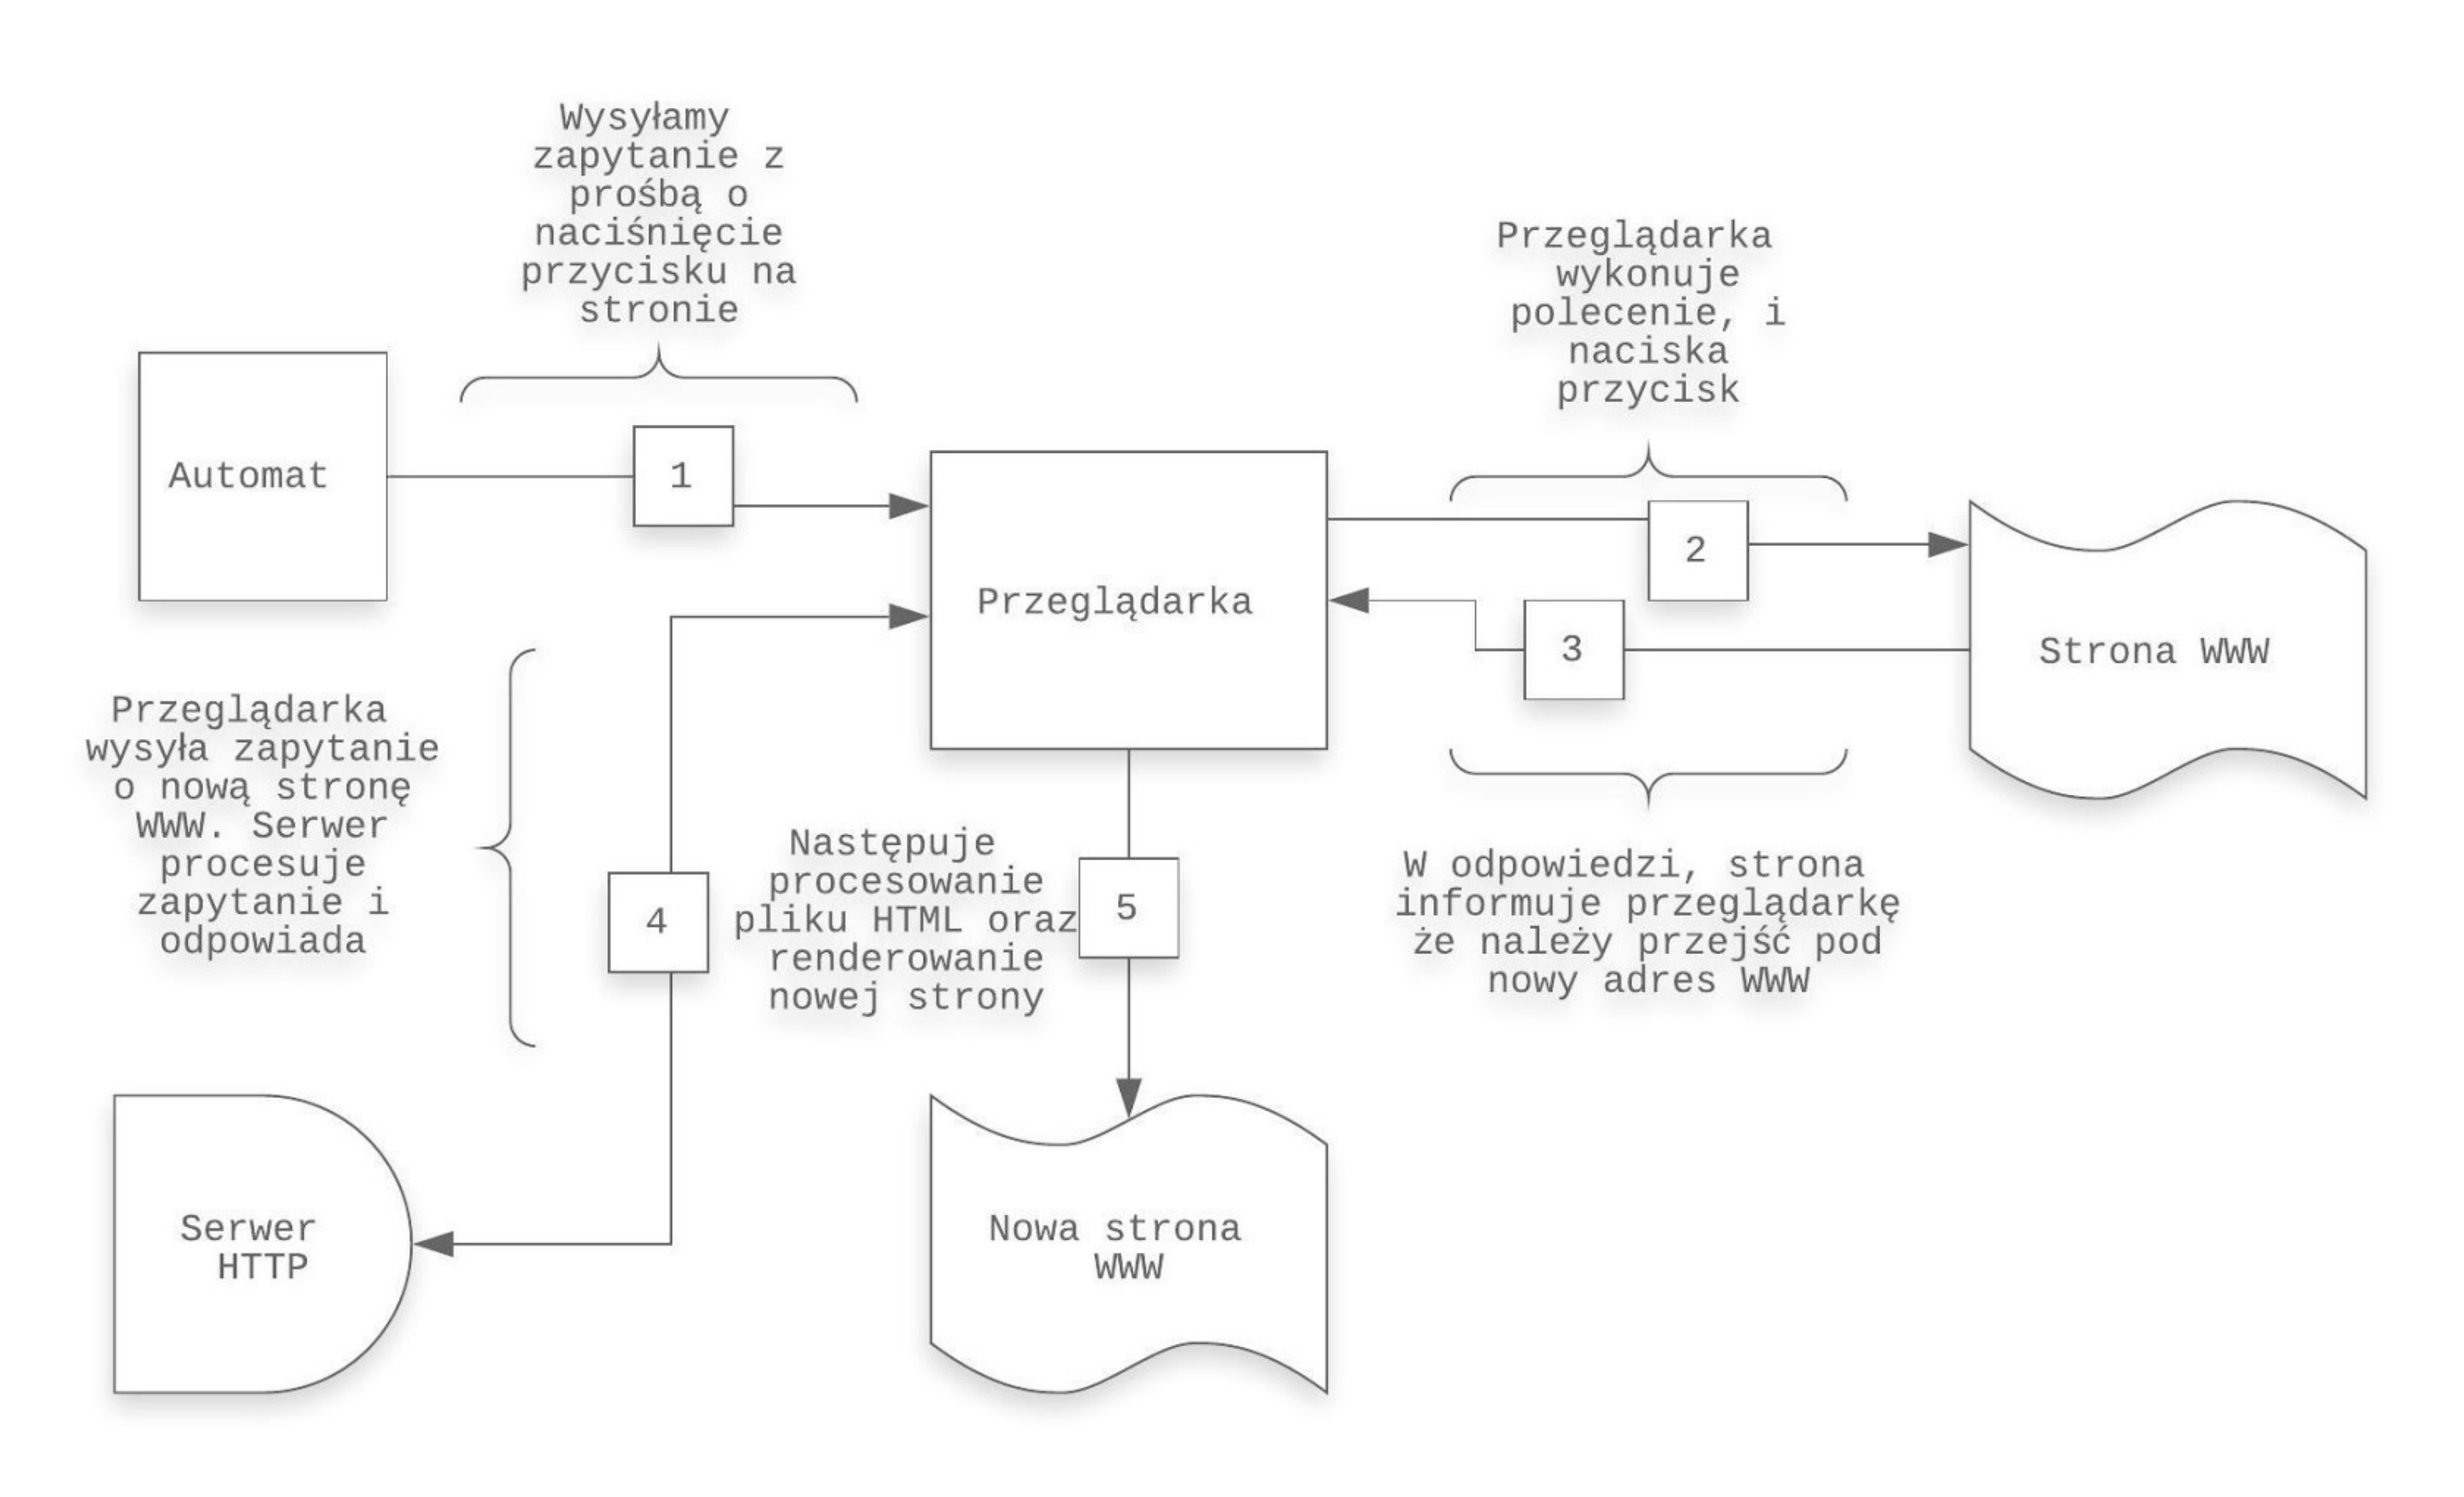
\includegraphics[width=12cm]{rysunek_19.png}
    \caption{Grafika przedstawiająca proces przeładowania strony statycznej}
    \label{fig:rysunek_19}
\end{figure}

\begin{figure}[!ht]
    \centering
    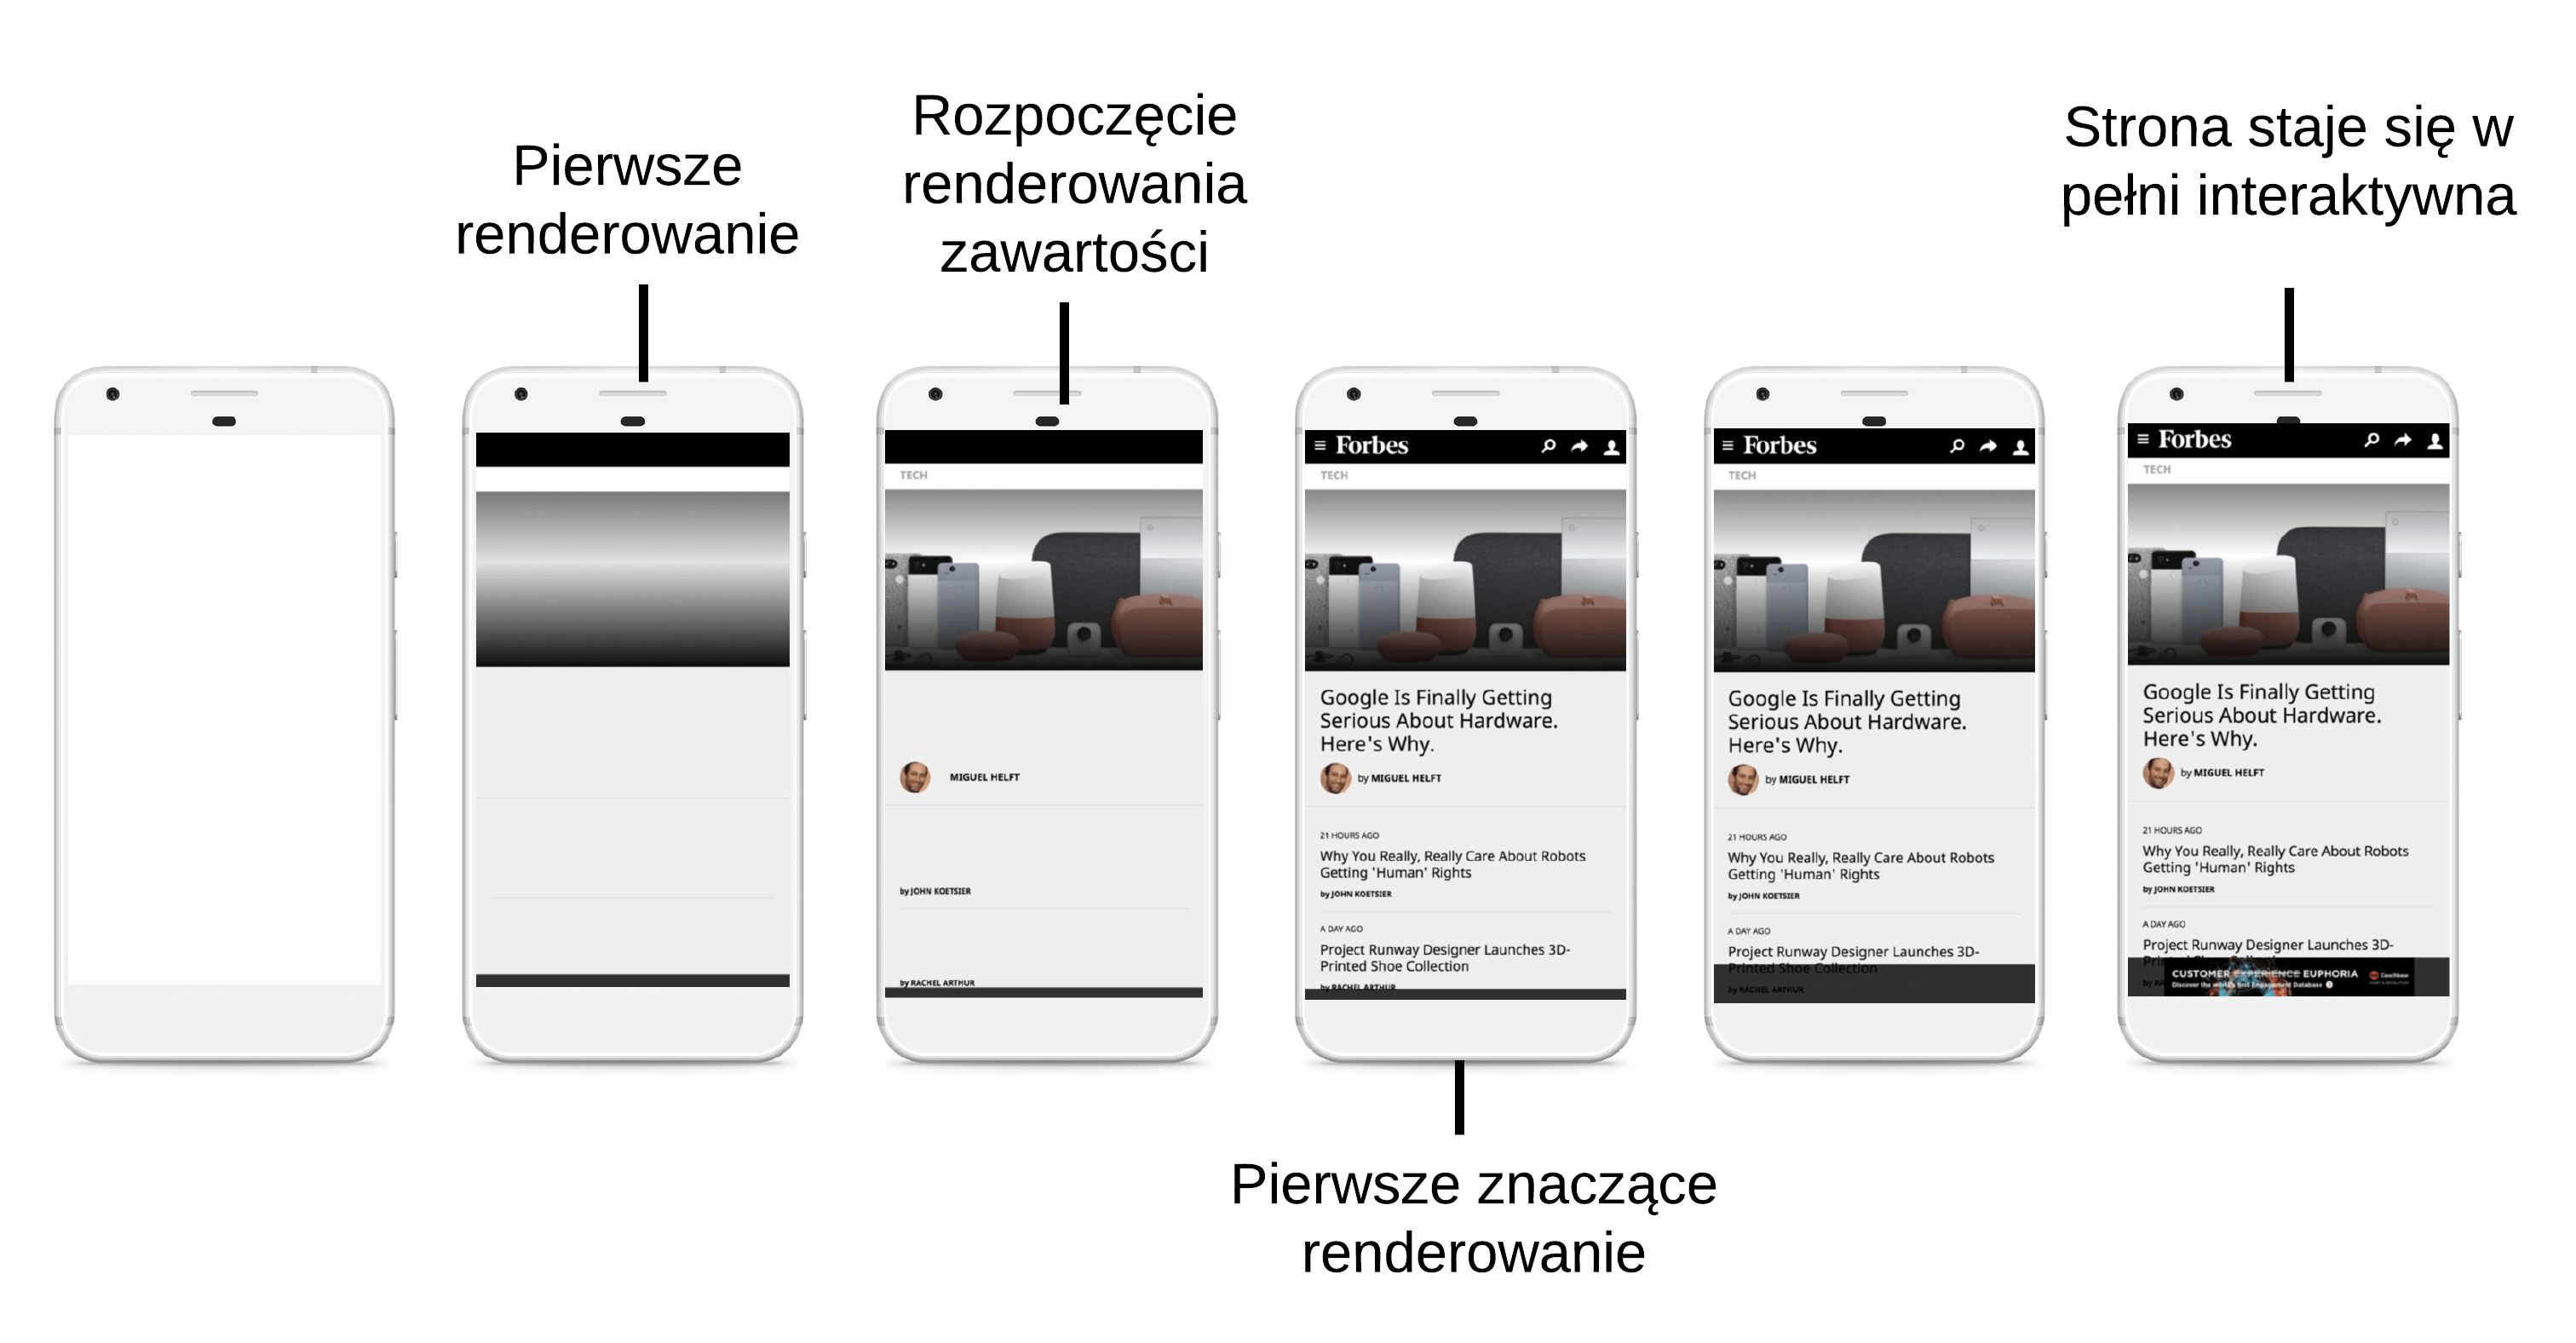
\includegraphics[width=12cm]{rysunek_20.png}
    \caption{Ilustracja procesu ładowania aplikacji oraz zdarzenia rejestrowane przez przeglądarkę}
    \label{fig:rysunek_20}
\end{figure}

\begin{figure}[!ht]
    \centering
    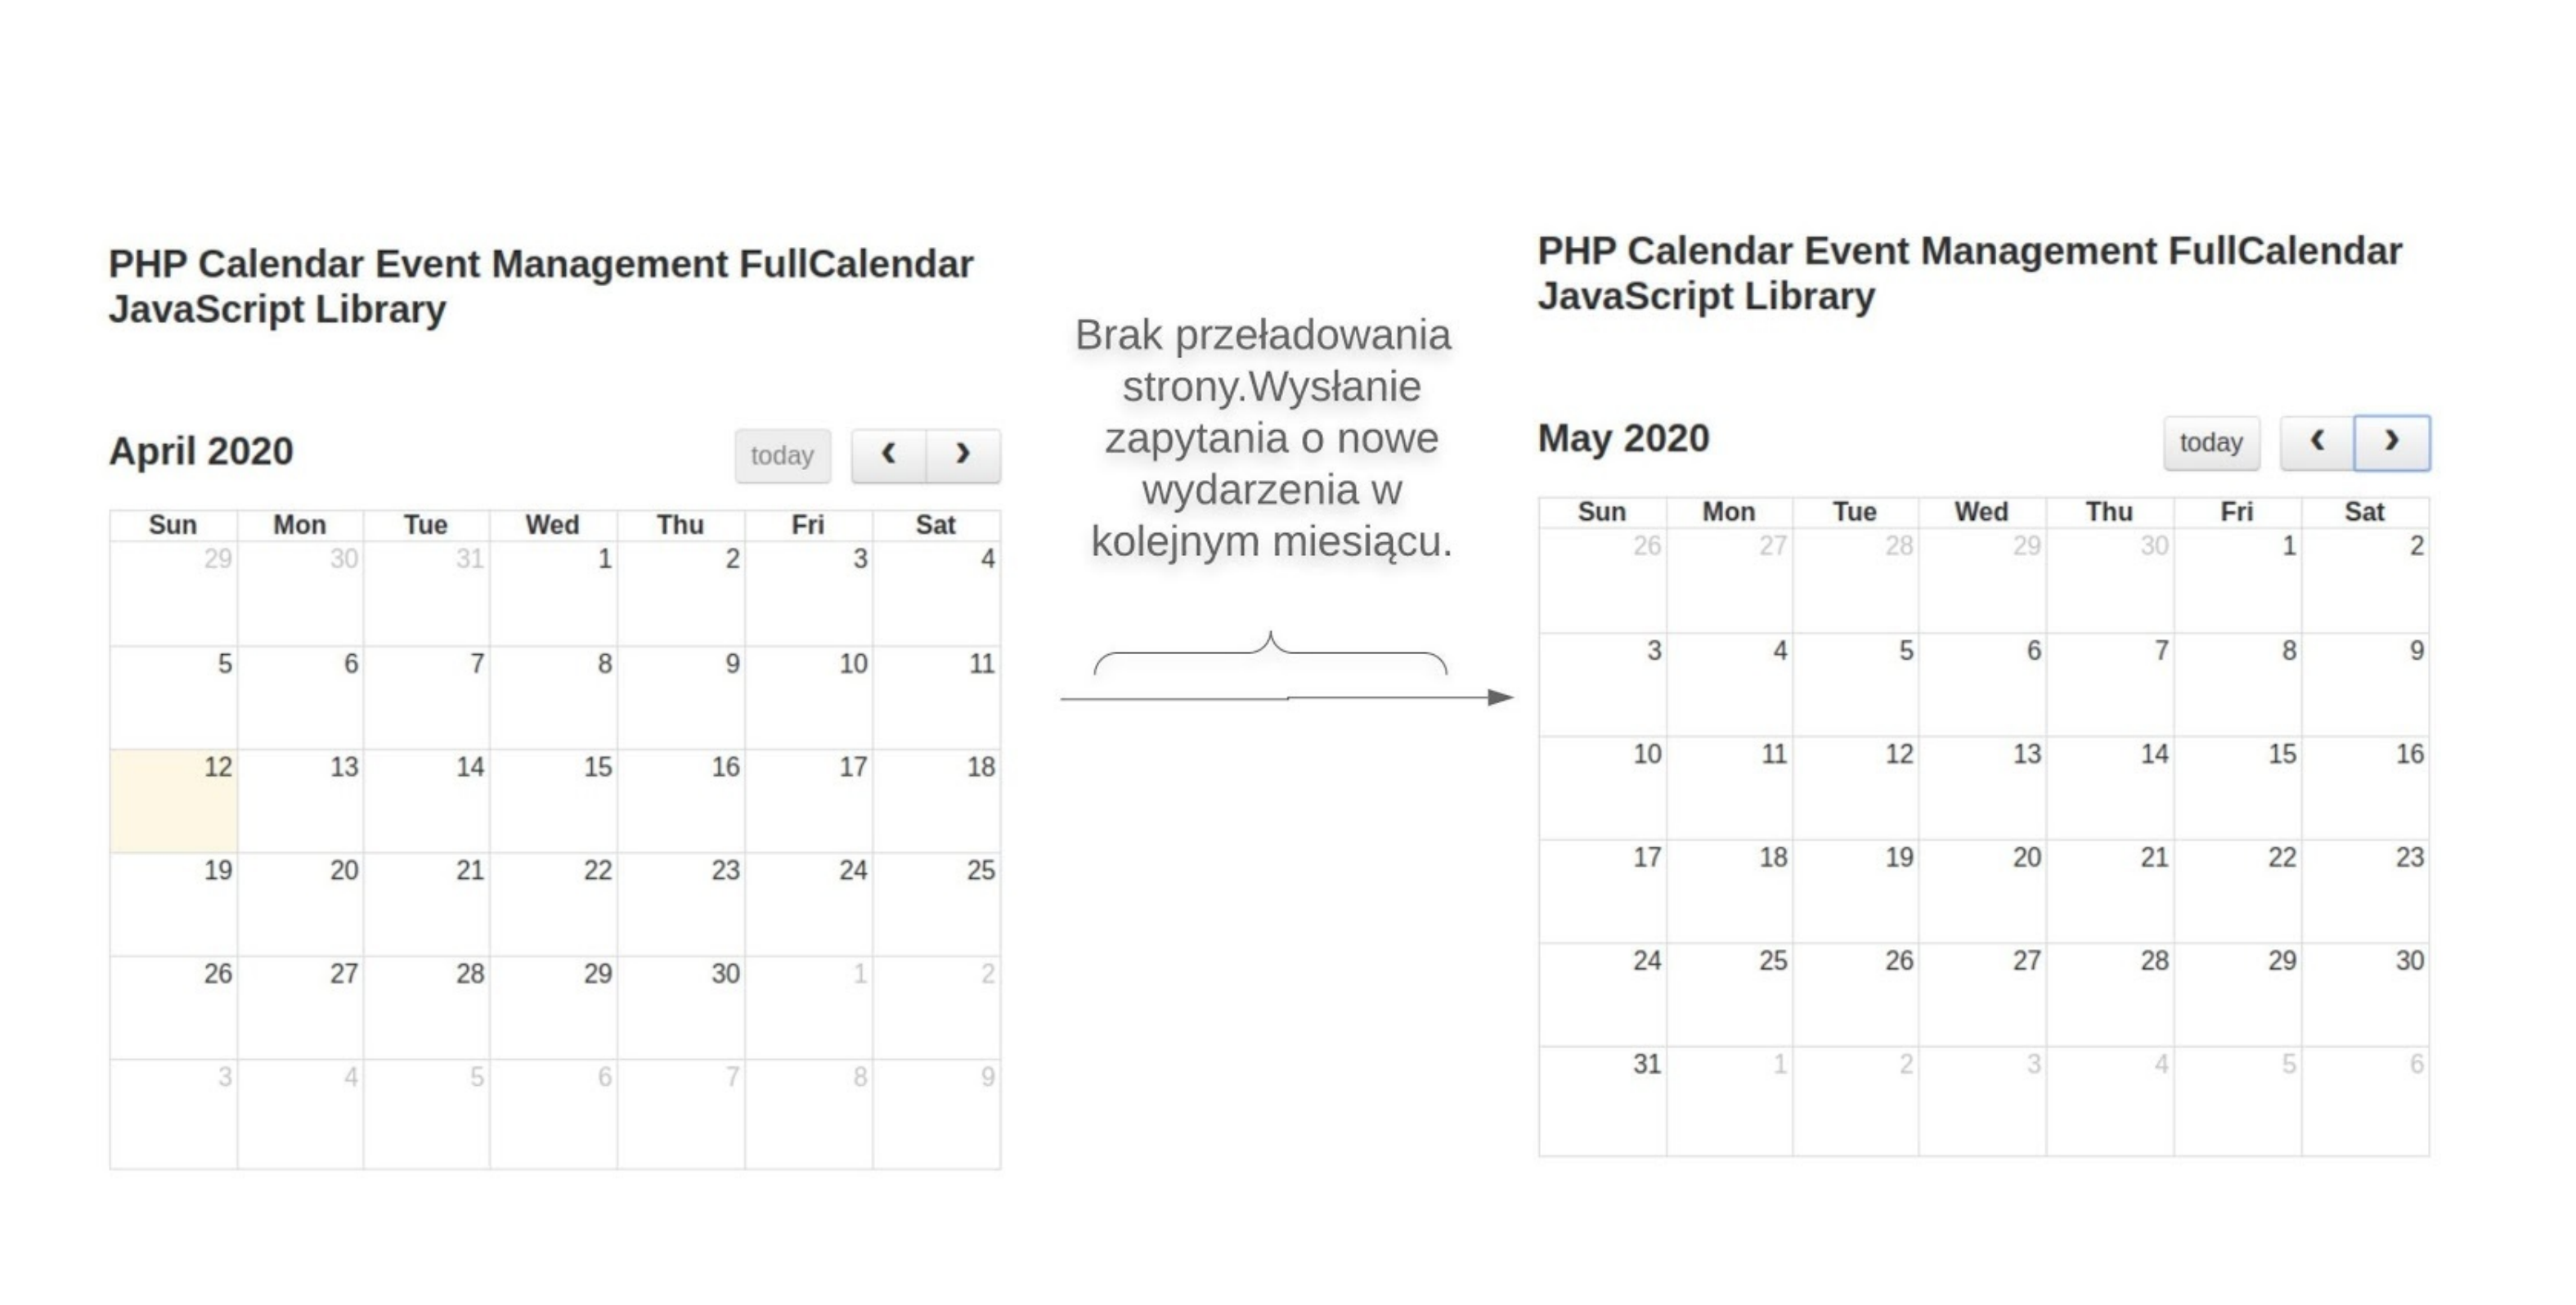
\includegraphics[width=12cm]{rysunek_21.png}
    \caption{Ilustracja mechanizmu zmiany daty w przypadku aplikacji dynamicznej}
    \label{fig:rysunek_21}
\end{figure}

%czyści puste strony
\let\cleardoublepage\clearpage